\documentclass{article}
\usepackage{graphicx}
\usepackage{amsmath}
\usepackage{amsthm}
\usepackage{amssymb}
\usepackage{geometry}
\usepackage{subcaption}
\usepackage[style=numeric,bibstyle=numeric,backend=biber,natbib=true,maxbibnames=99,giveninits=true,uniquename=init]{biblatex}
\usepackage[utf8]{inputenc}
\usepackage{amsmath}
\usepackage{algorithm}
\usepackage{algpseudocode}
\usepackage{hyperref}

% for the flowchart
\usepackage[dvipsnames]{xcolor}
\usepackage{tikz}
\usetikzlibrary{shapes.geometric, arrows}
\usepackage[skins]{tcolorbox}

\tikzstyle{nnmodel} = [trapezium, draw=black, fill=blue!20, trapezium left angle=120, trapezium right angle=120]
\tikzstyle{textcontainer} = [rectangle]
\tikzstyle{imageframe} = [rectangle]
\tikzstyle{arrow} = [thick, ->, >=stealth, draw=Maroon]
\tikzstyle{nonactivearrow} = [thick, ->, >=stealth, draw=Maroon!30]

\usetikzlibrary{positioning}

\addbibresource{../bibliography.bib}

% options: change 'markings' to 'entries'? include 'handwritten'?
\title{Fine-tuned Optical Character Recognition for Dental Fossil Markings}

\begin{document}

\tableofcontents

\section{Abstract}

Digitizing and uniformizing the structure of handwritten fossil catalogues exhibits a great 
potential for increasing the accuracy of paleontological data analysis by increasing sample sizes. 
Approximately 90, 000 of such samples reside in the archives of the National Museums of Kenya, and 
an ongoing effort is to store this data in a digital format for better accessibility.
A previous project utilized a commercial optical character recognition service for automated reading of these catalogues. This generalist
handwriting detection model lacked the ability to detect special characters used to denote tooth samples,
 leading to loss of information and detection mistakes.

This thesis proposes a classifier chain approach for detecting which tooth is shown on an image of tooth marking 
and a pipeline for using this tool for uniformizing the dental notation present in 
the bone or tooth type specifying column. The best base model is searched by comparing multiple convolutional and transformer architectures
to classify notation to upper or lower jaw, with the best accuracy of 96\% using AlexNet. 
In the experiments it is found that the quality of optimum found in training affects end results significantly,
leading to margins of error up to 10\% for architecture comparisons in a small data case.
The most clear result is that not freezing layers, without exception, leads to better result.
Because of this it is theoretisized that the utility of transfer learning mostly comes from 
being able to train more rather than being able to re-use a feature extractor.
The pipeline with best-performing classifiers based on the experiments is used to
to obtain an accurate reading of the catalogues of the National Museums of Kenya, and the tool is published to be used 
by the paleontological community for further digitization efforts.

Keywords: Optical character recognition, Transfer learning, Paleontological databases

\section{Introduction}

% outline of an introduction
% introduce the broad research area, why this is interesting. 1-2 paragraphs. context, anyone should be able to understand.
% first sentences: state the topic clearly
% broad research area: paleontology: data analysis on fossil finds
% dig fossil from the ground. identify:which bone,species,time. write this on a field slip, a slice of
% baking sheet like paper 
% analysis: take set of fossils, use methods for deducing eg climate, habitat, vegetation
% why this is interesting 
%     reactions of ecosystems to climate change
%     what ancient worlds were like 
%     how ancient humans lived
%     mass extinction events

The field of paleoecology conducts data analysis on fossil specimens.
Such analysis is quite literally started from the ground: after a fossil specimen has been found, it is 
carefully measured and identified: which bone and species the fragment is from, and how old it is. On site, such information is logged on field slips, small thin sheets of 
paper with a pre-printed form. The analysis has then been traditionally conducted by 
collecting such entries, sometimes collected in handwritten tabular catalogues, and running statistical 
tests on the sample set. With this analysis, facts from distant past, such as climate, habitats and 
vegetation can be deduced~\cite{Faith_Lyman_2019}. Syntheses of such results consequently allow us to 
answer larger questions, such as how ecosystems reacted to climate changes, how mass extinction events 
came about, and what the living world could be like~\cite{Zliobaite2023}. Understandably, answering such 
questions has become ever more pressing.

% now we have a stack of baking sheets in a room in kenya.
% paleontologists form all over the world want to solve climate change, among other problems
% big data methods would explode what paleoecology can do
% so we need to put the baking sheets on the computer to do analysis on big data
% what is the topic of my work?
% the baking sheets contain weird characters that a normal reader cannot read.
% my topic is to read them

To find answers to large-scale problems, more sophisticated computational data analysis methods have come about,
relying on large datasets. Due to the infeasibility of collecting stacks of fields slips across sometimes multiple 
continents, specimens residing in archives of institutions have been converted to digital, public databases.
One such institution is the National Museum of Kenya, holding a large fraction of data collected from one 
of the most valuable fossil sites globally, the lake Turkana. The sheer amount of physical samples in the museum storage
makes keeping them safe a significant challenge, a risk to global heritage now attracting attention across continents,
 as reported by the Wall Street Journal~\cite{hotzMuseumOverflowingPrehistoric2024}.
 A project digitizing the handwritten catalogues hosted by the NMK was started by
using commercial optical character recognition software, combined with heuristic and machine learning approaches, 
resulting in satisfactory accuracy on conventional handwritten text. However, a large hurdle in the existing 
approach were the special characters used to denote which teeth each specimen contains. The aim of this work is 
to continue the project by digitizing these markings accurately.

% explanation of the specific problem
%given scanned images and data with bounding boxes of sentences and words where tooth denoting words are 
%badly read, how can tooth element recognition results be improved? Goal is to have both this is what the element 
%/ nature of specimen column says (eg example here) and what/which teeth are found in this specimen in standardized format
%(eg example here)
%the topic of my work is creating a tool that inputs cropped images from the sheets containing
%handwritten specifications of fossil bones and outputs what the text says

Specifically, this work uses as input data both scan images of the fossil slips and catalogues, 
and outputs from the Azure AI Vision software~\cite{azurevision}.
The existing outputs consist of sentence and word-level readings, along with bounding boxes defining 
the location of each word or sentence. The main research question is the following: 

How, given scan images, bounding boxes and generalist OCR outputs, can the accuracy of the readings of the tooth markings be improved?

% 1. the pipeline + experiments
% (solution and previous analogous solutions)
% classifier chain
% image & azure output
% tooth or not based on azure output
% if not tooth keep azure output
% else feed to classifier chain, one tells tooth type from marking image, one index number, one up/low jaw
% combine tooth info & concat
% best is alexnet, no freezing with test acc ... in uplow.
% fraction of teeth class confidence over 99.7 so no manual verifying for each submodel: x-y%
% take min less certainty is limitation but still is found that this approach works, classifier accuracies are worst 88 best 100
This thesis proposes a univariate classifier chain approach for 
uniformizing the dental notation. Each element description is processed 
word-by-word and for each word only those recognized as tooth markings, 
by using a regular expression on the Azure reading, are given to the tooth 
classifiers. This way, more complex cases are left unprocessed, a desirable
approach as this is one of the first works attempting automated cleaning 
of digitized fossil data. The images recognized as tooth notation are given 
to three classifiers: first one detects the letter on the image to a 
tooth type, second detects whether the tooth is from the upper or lower jaw,
and third recognizes the index number. Finally, all these inferences can 
be combined to tooth notation and concatenated to a corrected element 
description. 

In the experiments for building the univariate classifiers, various base models and training configurations are compared, and 
AlexNet with no layer freezing is found to result in best test accuracy of 92.31\% on the 
upper or lower jaw classification task. However, it is found that different hyperparmeter 
configurations influence the scores by up to 10\%. 
Fractions of test images classified correctly with above-99.7\% confidence are 
counted to estimate the amount of saved manual verifying effort with these scores ranging 
from 58\% to 94.5\% depending on the classification task.
The approach of annotating a dental marking with the minimum 
confidence of all classifiers causes most of the final confidence scores 
to be too low to bypass manual verifying, thus it is possible that little manual labor is 
saved with this initial solution. Still, it is proved that the proposed approach works and that 
accurate classifiers with test accuracies ranging from 88.0\% to 100.0\% can be built 
with the techniques implemented.

% relevance for other work: why was this specific problem? how can this be concretely used?
% relevance of this work: KNM is able to have way more precise dental element markings
% to other catalogues: previous project + this a complete solution to digitizing the handwritten data 
% relevance of this work: any field that does:
% - ocr on unconventional characters
% - ocr where each character has a multivariate output (eg. this is an a. it is underlined could be letter and underlined /not underlined)

The direct impact of this work is an improved precision of the tooth element entries in the digitized 
fossil catalogues of the National Museum of Kenya, but the results are applicable to a wider domain of problems.
Intuitively the results are directly applicable to other fossil archives using similar notation: only a fine-tuning of the 
models to the new archival data is necessary.
For other handwritten archives, the results presented can be used to improve recognition accuracy, especially in cases 
where the data contains characters other than latin letters or arabic numerals. Additionally, this work presents
a potential solution for when the target character set can be expressed with multivariate output data. This could, for 
instance, be handwriting with occasional underlinings, where the bivariate output could be the letter and a boolean variable for 
whether the character was underlined.

% organization
The rest of this thesis is organized as follows. First, the necessary background theory is 
presented. For paleoecology, the background covers 
foundational ecological laws followed by a brief introduction to methods used in
paleoenvironmental reconstruction, especially focusing on inferences from tooth data,
followed by a presentation of the mammal tooth row.
For deep neural networks, the following concepts are introduced:
the basic network structure, how training is conducted, basic building blocks of character-recognizing network architectures, and transfer learning. 
Second, related work is presented, both on
handwritten archive digitization and transfer learning with character-recognizer models.
Next, the experimental setup is introduced, covering dataset creation, labeling and data 
preprocessing, followed by base model and transfer learning method selection. After this, 
results of the experiments are presented and discussed. Finally, the work is concluded.

\section{Fundamentals on paleoecology}

% start: what is this field about 
%paleoecology is data analysis on fossil data
%most common application: paleoenvironmental reconstruction
%    definition of the problem: whan ancient habitats were like and what changes they 
%    underwent at which times (ch2)
Paleoecology is a field that conducts data analysis on fossil specimens. The most common type of 
this analysis is paleoenvironmental reconstruction: deducing what past habitats were like and which 
changes they have undergone~\cite{Faith_Lyman_2019}.

%abstract how analysis is done (species to env map w present apply to past)
%basic process: learn fossil data to environment statistical relationship in present
%(study tolerances of animals ie in what kinds of enviroments animals live), apply to past 
%  tolerance = range of an environmental variable that is hospitable for the species~\cite{Faith_Lyman_2019}
%note on caveats ie what about this is difficult
%we need correlations but even those are hard: something correlates in present might not correlate in past
%Nature is highly complicated -> models and assumptions enable drawing conclusions from animal communities
%one needs to be super careful to draw conclusions, lots of evidence always needed
The high-level process for reconstructing paleoenvironments is to find a relationship between traits of an 
animal or plant community living in an area in the present time, and use this 
relationship to map sets of species in a fossil assemblage to paleoenvironmental variables.
Traditionally, these relationships are constructed with expert knowledge on each species: The environmental conditions of
each species is studied independently and limits known as tolerances are learned. These sets of tolerances form niches,
the set of possible environmental conditions a species can live in~\cite{Faith_Lyman_2019}. Finally, these insights are aggregated to 
draw conclusions on past enviroments based on which species occur in fossil finds in a given location and time.
Naturally, there are multitudes of variants for drawing environmental conclusions from fossil data based on 
tolerances and niches, and the methods have many caveats, thoroughly overviewed in~\cite{Faith_Lyman_2019}. The most major ones of these are that one always has to 
make assumptions, such as assuming that tolerances will not change over time, and aggregate information by for instance 
disregarding individual adaptations. Additionally, with a set of species and a big set of environmental signals provided 
by each species, drawing conclusions on multitudes of often partially conflicting signals is a challenge.

%chapter intro 
%sect 1 highlights dental ecometrics as a method for paleoenvironmental reconstruction
%to motivate the need for representative and accurate dental fossil datasets. As further background on the data, sect 2 presents the
%mammal teeth row along with relevant terminology.
This chapter overviews relevant background on paleoenvironmental reconstruction from the perspective of this thesis.
Section~\ref{sect:ecometrics} highlights dental ecometrics, a method for constructing mappings from dental elements to environmental traits to motivate the 
need for representative and accurate tooth fossil datasets. As further background on the data, Section~\ref{sect:mammal_teeth} presents the mammal teeth 
row along with related terminology.

\subsection{Dental ecometrics}
\label{sect:ecometrics}

%%what it is on high level: transfer functions
%a mapping from taxa to environmental variables -> know fossil assemblage, deduce environment
%  learned using machine learning / statistical models (ch9)
%    benefit instead of tolerances/niches: they have subjective interpretation problems (book ch 9)
Dental ecometrics is a method for constructing transfer functions, mappings from species occurences to environmental traits.
These can be learned using statistical models, such as regression, or classic machine learning methods.
Using transfer functions is considered more accurate than expert analysis on tolerances and niches: the latter
can contain subjective interpretations, and transfer functions allow analyzing much larger sets of species occurences than would 
ever be possible for a human analyst~\cite{Faith_Lyman_2019}.

%%what dental ecometrics is specifically, lophs and hypsodontry
%dental ecometrics = inference of transfer functions given dental data (ch9 liu et al 2012),~\cite{oksanenHumboldtianApproachLife2019}
%relation of traits of animals and livelihood = ecomorphology~\cite{oksanenHumboldtianApproachLife2019}:
%    teeth -> diet -> what plants grew and habitat -> climate etc
%example both fortelius and oksanenHumboldtianApproachLife2019:
%  dental lophs (cutting blades) and hypsodonty (crown height) to temperature and precipitation
%    two kinds of plants, browse (dry), grass (moist).
%    dominant molar, usually 2nd, primary chewer tooth
%    grass -> high-crowned ie hypsodont molars
%    browse -> dry plants need more blade-like molars ie more pronounced lophs
%    then you take the teeth, check hypsodontry and lophs of the species present, check occurences of species in regions 
%        statistical model (variants of regression usually) between teeth and present environment
%        use mapping to fossil teeth in the past -> get past temperature variables.~\cite{oksanenHumboldtianApproachLife2019} for instance got temperature, fortelius precipitation
%relevance to present eg find how much loss of tree cover affects temperature (fortelius)
%super relevant for forecasting whats to come with climate change
Dental ecometrics constructs transfer functions where the input variables are dental traits~\cite{Faith_Lyman_2019, oksanenHumboldtianApproachLife2019}.
The method is a subtype of ecomorphology; the study of the relation of functional traits of animals and plants with their livelihood
\cite{oksanenHumboldtianApproachLife2019}. The high-level reasoning behind the method is that teeth evolve to 
shapes that are most suitable for processing vegetation in the habitat, thus one can infer vegetation based on tooth shapes, 
which then serves as a good proxy for environmental conditions~\cite{oksanenHumboldtianApproachLife2019}. 
When the environment changes, animals have to move to habitats where the vegetation is digestible with their teeth, thus 
analysis on environmental change can be performed even on a smaller timescale than evolution would allow~\cite{fortelius}. As an example, both precipitation~\cite{fortelius}
and temperature~\cite{oksanenHumboldtianApproachLife2019} can be learned based on dental lophs, number of cutting blade shapes, and hypsodontry, the height of 
molar crown, with the following analysis. One can roughly divide available plants as grass, which has more water and is easier to chew, and 
browse, drier and rougher plants. The dominant molars are primarily used to chew these plants and it is known that to digest grass, a high 
crown is required due to tooth erosion and that to digest browse, cutting blades in teeth are required to cut the fibrous plants to pieces.
One can therefore find statistical relationships between these tooth measurements and environmental conditions that are favorable 
for the growth of grass or browse. Then, one can collect a large number of fossilized molars, measure the crown heights and blade shapes to construct a data set of 
tooth types found in a region during a set geological time period. The previously learned function can then be applied to this data set
 to get knowledge on environmental conditions. These insights on 
 past environments and how habitats interacted with their changes can 
 in turn be used to inform the present situation: for example, it can 
 be predicted how much local ground temperature rises when tree cover is lost~\cite{fortelius},
 and information like this is crucial in understanding the processes occurring with climate change.
  Again, the true relationships are naturally much more complicated 
 than the straightforward thought process presented here, but the rough idea is accurate.

% data precision/availability considerations
% -> what this means for data requirements
%data is needed for finer resolution (fortelius)
%is in many cases the limiting factor (faith lyman, fortelius)

%gathering data seems hard analytical papers have to eg measure the crowns before they can analyze (eg fortelius)
%-> pain, should be easier
%it seems that digital availability and nonuniform representations are a major limiting factor in 
%getting more precise insight

%so, getting more data is super important and even so more in my case:
%the turkana basin where my data is from: 
%theres human evolution (forteloius) and especially dense mammal record (fortelius) and many environmental changes (nowdatabase)

Many studies on paleoenvironmental reconstruction list data availability as one of the most major limitations~\cite{oksanenHumboldtianApproachLife2019 fortelius}.
As geoglogical time spans are huge, studies have to 
resort to time resolutions of hundreds of thousands of years (eg.~\cite{fortelius}) because of a lack 
of sufficient sample sizes. It seems that one of the major hurdles in verifying a hypothesis on 
paleoenvironments is the effort required to collect and curate a dataset; for instance, some ecometric
analysis works start by measuring the dental traits~\cite{fortelius}, an effort that could be saved 
if measurements were collected once and then stored in a structured manner. For this reason, the 
creation and maintenance of paleontological databases is of central importance, and this is accentuated 
in the case of the Turkana basin, for which most of the data points are stored in catalogues processed in 
this work: it is suspected that
important steps in human evolution occurred there, the mammal record is especially dense~\cite{fortelius}, and the area has undergone many environmental transitions in the past~\cite{Žliobaitė2023}.

The goal of this work is to advance automated curation of paleontological databases, 
with the primary aim that the structured, digital data would allow for 
more accurate analysis thanks to larger samples and less tedium in 
setting up experiments. The terminology special to fossils present in 
the curated data is presented next.

\subsection{Composition of mammal teeth}
\label{sect:mammal_teeth}

%Fossils occur when animal / plant remains are deposited in a sediment in a way that preserves 
%some part of its original form. Since teeth are the hardest material in animals, large fraction
%of found parts are teeth. Fossil finding is followed by identification to most specific taxon possible
%largely a technical skill (ch5), teeth are identified down to type and number, how manyeth the teeth are,
%counting from center to edge or other way round??
%specimen can be either one tooth or fragments of the jaw bone where there are multiple teeth (markings like M1-3)
% present teeth here

Since geological events tend to erode organic remains the faster the remain decomposes, the hardest materials in 
the corpse represent largest fractions of fossil datasets. These hard materials include shells, bones and especially teeth, and 
the last is prominent in fossil data analysis also due to the fact that they encode a diverse set of information on 
the livelihood of the organism~\cite{Faith_Lyman_2019}. The identification of the fossil remain is done at the finest resolution possible,
preferring taxon information over just identifying the genus, for instance. Finest-resolution information 
derived from dental fossils are the taxon the tooth is from, and which tooth or teeth are found in the specimen.
This section presents the naming and indexing system for mammal teeth commonly used in paleontological datasets,
as described by Hillson~\cite{Hillson_2005}, and some common shorthand versions present in the dataset digitized in this work.

% complete jaw-describing terminology
% the jaw bones
%lower jaw bones: mandibles, upper jaw: maxilla, premaxilla
% permanent and deciduous (D), nonpermanent "milk" teeth (laita vaan jos löytyy d-hampaita)
Specimens including more complete fragments of the jaw are described with terminology related 
to the jaw bones. All mammals share the same bone structure around the mouth: the lower jaw consists 
of two bones called \textit{mandibles}, joining in the middle, whereas the upper jaw consists of bones called 
\textit{maxilla} and \textit{premaxilla}, that also form large parts of the face.
A common trait across many mammals is also that the permanent teeth erupt in the 
youth of the animal, replacing the 'milk' or \textit{decidous} teeth. Shorthands commonly used for these 
terms are 'mand' for mandibles, and capital letter 'D' for the decidous teeth.

% types of mammal teeth
%four classes, front to back: three incisors (I), one canine (C), four premolars (P), three molars (M). top bottom left right. top/bottom noting upper jaw as superscript lower jaw as lower script, 
% purpose: incisor -> catching, canine -> stabbing / killing prey, molars are for chewing. premolars are bit like canines bit like molars, function varies lot
% between taxa including holding, cutting and chewing. also form and number of each present changes between taxa.
%sometimes lower jaw as line on top and upper jaw as line on bottom, sometimes both are used: upper script number with line on bottom. Line is "the other jaw"
%if there are less of a type of teeth eg two premolars, they might be no 1 and 2 or no 3 and 4
The tooth rows of mammals are classified to four classes; \textit{incisor}, \textit{canine}, \textit{premolar}
and \textit{molar} and indexed with a numbering system. Moving from the middle of the tooth row
towards the side, there are up to three 
incisors, used for catching food and denoted with the letter 'i'. Behind them is the canine tooth, used for cutting, and 
in case of predators, killing. This tooth is denoted with the letter 'c'. Behind the canine are up to four premolars, noted with 'p'. These 
teeth vary most between taxa in form and function with functions including cutting, holding and chewing food.
The teeth at the back of the row are called molars, 'm', and are primarily used for chewing. Molars, like the other tooth types, 
vary in number between taxa, and are at most three. The numbers are always increasing when moving back in the tooth row, but in
 the case of missing teeth in a taxon, the numbers do not necessarily start from one: instead, the number is chosen to 
have teeth with same numbers as alike each other as possible. Thus, a taxon with only two premolars might only have the teeth P3 and P4.


% directional terminology
% distal "far from center of body", proximal "close to center of body", mesial "close to mouth opening"
%right and left sides are always symmetrical, denoted simply L or R or Lt or Rt or left or right. left is left looking from the animal, not the observers perspective
Location of the tooth present in the fossil is described with directional terms specifying the side, jaw and the location on the jaw.
The most
intuitive are left and right describing the side, where one needs to note that each denotes the side from the viewpoint of the 
animal, not the observer. Mammal teeth are always symmetrical, thus every tooth always has the 
equivalent other-jaw counterpart. The distance of a tooth from the throat 
is described with the terms \textit{distal}, 'far from to the mouth' and \textit{mesial}, 'close to the mouth'. For skeletal bones, the term \textit{proximal}, 
'close to the center of the body' is often used instead of 'mesial'.
Short-form versions for these terms include capital 'L' or 'Lt' for left, capital 'R' or 'Rt' for right, 'dist.' 
for distal and 'prox' for proximal.
The jaw, upper or lower, has three dominant notation styles: one is to sub- or superscript tooth index numbers, other is to 
over- or underline tooth markings, and the last style, prominent in digital fossil data, is to set the tooth type letter to upper- or lowercase.
In each of these systems, a superscipt, underline, or capital letter denotes upper jaw, and conversely subscript, overline or lowercase letter denotes the lower jaw.
An illustration of the mammal tooth system is presented in Figure~\ref{image:mammal_teeth}. Terminology with corresponding shorthands are summarized in Table~\ref{table:terminology} and jaw notation styles in Table~\ref{table:jaw_notation}.

\begin{figure}[h]
    \centering
    \includegraphics*[scale=0.43]{../images/teeth_img_hillson_book.png}
    \caption{Mammal teeth composition, from Hillson~\cite{Hillson_2005}.}
    \label{image:mammal_teeth}
\end{figure}

\begin{table}[ht]
    \centering
    \begin{tabular}{|l|l|l|}
        \hline
        \textbf{Term}       & \textbf{Meaning}                                   & \textbf{Shorthands}       \\ \hline
        Mandible            & Lower jaw bone                                     & mand.                     \\ %\hline
        Maxilla, Premaxilla & Upper jaw bones                                    &                           \\ %\hline
        Deciduous           & 'Milk teeth'                                       & D, d                      \\ %\hline
        Incisor             & Tooth type (front, middle)                         & I, i                      \\ 
        Canine              & Tooth type (between incisor and premolar)          & C, c                      \\ %\hline
        Premolar            & Tooth type (between canine and molar)              & P, p                      \\ %\hline
        Molar               & Tooth type (back of tooth row)                     & M, m                      \\ %\hline
        Distal              & Far from body center / mouth                       & dist.                     \\ %\hline
        Mesial              & Close to the mouth                                 &                           \\ %\hline
        Proximal            & Close to body center                               & prox.                     \\ \hline
    \end{tabular}
    \caption{Terminology related to mammal teeth with corresponding shorthands}
    \label{table:terminology}
\end{table}

\begin{table}[ht]
    \centering
    \begin{tabular}{|l|l|l|l|}
        \hline
        \textbf{Jaw}      & \textbf{Line Notation} & \textbf{Sub/Superscript Notation} & \textbf{Digital Notation} \\ \hline
        Upper         & $\text{M}^{\underline{1}}$      & m\textsuperscript{1}              & M1                        \\ 
        Lower         & $\text{M}_{\overline{1}}$ & m\textsubscript{1}                & m1                        \\ \hline
    \end{tabular}
    \caption{Dental marking styles, Example: first molar. Line notation displayed in common style combining sub- and superscripts.}
    \label{table:jaw_notation}
\end{table}

% summary of chapter ???
This chapter overviewed background on paleoenvironmental 
reconstruction to motivate the necessity for structured paleontological 
databases. Additionally, terminology present in the data processed was presented.
The next chapter presents background theory on deep learning, which is required for data 
uniformizing processes completed in this work.

\section{Deep neural networks for optical character recognition}

% introduction to chapter
% point of this section: present relevant deep learning theory
% running example: reading characters from images (optical character recognition, OCR)

This chapter presents relevant background on deep neural networks (DNN), also known 
in literature as artificial neural networks (ANN) or, for historical reasons, multilayer perceptrons (MLP).
The aspects presented are constrained to those relevant to the problem at hand, optical character recognition (OCR),
that is also used as a running example.

\subsection{Deep neural networks}

% what is a neural net
% yes what is a neural network? function?
% weights in layers: floating point numbers, grouped in groups 
% activations: connections between weights, nonlinear scalar to scalar functions 

Neural networks are multivariate functions that share a specific form.
The function parameters, usually floating-point numbers, are called weights and are organized in groups called layers.
The first layer is called the input layer, after which there are multiple hidden layers, followed by the output layer.
Weights of adjacent layers are combined by activation functions, that are constrained to nonlinear functions with 
scalar inputs and outputs~\cite{princebook}. Simplest of the activation functions is the rectified
linear unit ReLU, shown in Equation~\ref{eq:relu}. A neural network is usually visualized with a graph structure, as seen in Figure~\ref{image:neuralnet}, where a node represents a 
weight, and an edge denotes that the value on the first layer is used to compute the value on the latter.

\begin{align}
    \text{ReLU}(x) = \max(0, x)
    \label{eq:relu}
\end{align}

\begin{figure}[h]
    \centering
    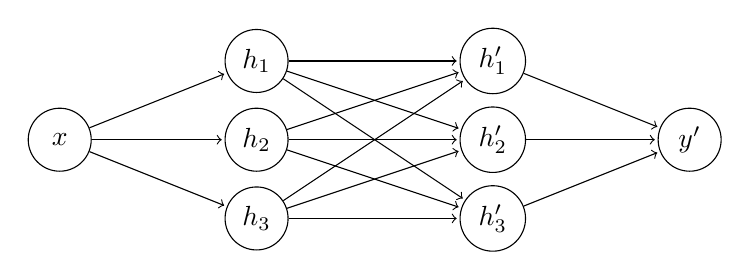
\begin{tikzpicture}[->, shorten >=1pt, auto, node distance=1.5cm, main node/.style={circle, draw, minimum size=0.8cm}]

        \node[main node] (x) {$x$};
        \node[main node] (h1) [right of=x, xshift=1cm, yshift=1cm] {$h_1$};
        \node[main node] (h2) [right of=x, xshift=1cm] {$h_2$};
        \node[main node] (h3) [right of=x, xshift=1cm, yshift=-1cm] {$h_3$};

        \node[main node] (h1') [right of=h1, xshift=1.5cm] {$h_1'$};
        \node[main node] (h2') [right of=h2, xshift=1.5cm] {$h_2'$};
        \node[main node] (h3') [right of=h3, xshift=1.5cm] {$h_3'$};

        \node[main node] (y) [right of=h2', xshift=1cm] {$y'$};

        % Edges
        \foreach \i in {1, 2, 3} {
            \draw (x) -- (h\i);
            \draw (h\i) -- (h1');
            \draw (h\i) -- (h2');
            \draw (h\i) -- (h3');
        }

        \foreach \i in {1, 2, 3} {
            \draw (h\i') -- (y);
        }
    \end{tikzpicture}
\caption{Visualization of a neural network with scalar input and output, and two fully connected layers, redrawn after~\cite{princebook}.}
\label{image:neuralnet}
\end{figure}

% - feed forward
% network computes output from input with the feed forward.
% you have an input, bunch of numbers
% then, you compute a linear combination and pass that through an activation function 

The computation of an output based on an input in the network is called the 
feed-forward, as the computation runs forward layer by layer through the 
network. The process starts from the input layer, which is simply the input 
organized as a vector. Each intermediate value on the first hidden layer, noted $h_d$ below,
is computed by taking a linear combination of the layer weight vector $\mathbf{\theta}$ and 
the input vector $\mathbf{x}$ of size $N$, adding the 
bias term $\theta_0$, and passing the result through the activation function $a$:

\begin{align}
    h_d = a\left[ \theta_{0} + \sum_{i=1}^{N}\theta_{di}x_{i} \right]
\label{eq:fc_layer}
\end{align}

% mean that this computation is done in a different manner (conv, transformer)
Different types of layers, such as convolutional or transformer layers 
denote that this single-layer computation process is performed differently from 
the standard form. When many layer types are present, layers using the computation
in Equation~\ref{eq:fc_layer} are called fully connected or dense layers.

% a is any nonlinear funtion, simplest is the rectified linear unit relu, x=x if x>0, x=0 if x<0.
% hidden units are taken as inputs to next layer and next and next. thetas = weights
% largest, deepest: hundreds of layers, hundreds of millions of weights 
% then last hidden unit output it the output of the network. tadaa.
The computation proceeds from the first hidden layer in a similar manner: 
the next layer values, also called activations, are computed using the weights of 
the layer and the previous layer activations with Equation~\ref{eq:fc_layer}.
The activations of the output layer is the output of the network.
More complex networks are generally constructed by increasing the network size to up to 
hundreds of layers with hundreds of millions of parameters, and by using
different types of layers.

% - universal function approximator
% the theory of the universal approximation capacity: this algebraic construct, 
% given correct weights, activation functions and structure, could approximate 
% any mapping from input to output. note: input/output dimension can be anything
The universal function approximator theorem states that functions belonging to the 
neural network family are capable of approximating any mapping from any type or shape of input
to any output with arbitrary precision~\cite{princebook}. Naturally, due to high computational 
costs of finding the optimal weights and the large search space of possible networks, 
this theoretical optimum is rarely reached.

% examples from ocr relevant in this case
% input is always image ie 2d matrix if grayscale or 3d tensor if rgb image.
Examples of input-output mappings relevant in this work are the following, 
ordered from simplest to most complex: tooth type classification, constrained multilabel classification, 
and sequence-to-sequence learning. The problem of tooth type classification takes in an input image of a dental marking
% this figure: see first all background & what samples are needed from tooth data...
 and decides which tooth the image denotes.
As mammals have up to eleven teeth on each side of two jaws, the classes would be 
these 44 teeth, such as 'rm1', 'lP4' or 'li2', using the computational notation presented in
Section~\ref{sect:mammal_teeth}. The network would output a 44-element discrete probability distribution 
obtained by using the softmax function (Equation~\ref{eq:softmax}), that takes as input the last layer output
values and returns an output layer vector of the same length but with values between zero and one and summing to one, 
thus a valid probability distribution.
Here, like in other classification tasks, each value notes the probability that the image contains 
the tooth this value is chosen to represent. The final output would then be the largest probability
found in this vector.

\begin{align}
    \text{softmax}_k[\mathbf{z}] = \frac{\exp[z_k]}{\sum_{k'=1}^{K} \exp[z_{k'}]},
    \label{eq:softmax}
\end{align}

% multilabel classification problem:
% image of tooth sample. output: first MIPC, second if it is upper or lower jaw
% output can be two arrays, one like before, other a 0-1 probability for upper jaw. upper if this > 0.5 
A better approach that could encode the fact that all teeth of same type share a similar input feature
, a letter in the image, could be formulating the problem as a multilabel
problem~\cite{multilabel_classification}: the output would be three of the aforementioned 
probability vectors, one with four elements representing 'M', 'P', 'C' or 'I', one with four elements 
for tooth indices, and two two-element vectors for left-right and upper-lower jaw. As this 
formulation lacks the notion that some tooth-type pairs never exist, such as the 4th canine,
this is a case of constrained multiclass classification, where some label pairs are marked 
as impossible combinations.

% present sequence to sequence learning:
% more complex case: image of sentence
% output: text on image, variable length. here output layer is a more complex 
% structure of probabilities for each position in the result sequence.
Generalizing the mapping problem further, one could also input a variable-length image 
of the entire dental marking comprising of multiple words, and outputting the text on this image.
Due to the variable output length, a special technique called sequence-to-sequence learning 
is employed~\cite{sutskever2014sequence}. This encodes the fixed-length output layer to variable-length 
output text. Even though all of the problems presented in this section recognize characters, 
generally the term 'optical character recognition' is used for this type of mapping. Models
for solving these problems accurately are very large, for instance the Microsoft TrOCR has approximately 
500,000 parameters~\cite{li2021trocr}.

Finding the best network weights for any of these types of input/output mapping problems, training 
a network, is conducted with the same process.
The general recipe for training a neural network is the subject of the next section.

\subsection{Training neural networks}
\label{sect:training}

% u have encoded the structure, starting weights. data, input/output pairs.
% training = process that adjusts weights so that network becomes a good 
% approximator
After one has defined a neural network structure, initialized the weights of the network 
to some initial values and obtained a sufficiently large set of input-output pairs from the problem at hand,
one can start training the network. Training is an iterative process where inputs are used to 
predict the output, which is then compared to the ground truth. A more detailed account of these iterations
is presented next.

% 1. take part of data as training data
% 3 divide to batches, common batch sizes are exponents of 2, 2-32 usually 
At the start of training, a small fraction, commonly 10-20\%, is reserved as test data. Cross-validation is 
generally not used with neural networks due to the computational cost of the training process (ref?). The remainder, 
the training set, is divided into batches, sizes of which are commonly exponents of 2.

% 4. pass a batch through the network. get output 
% 5. pass output and correct to loss function: map from output, correct to scalar,
% 0 is good, large value bad.
% 6. Compute loss function gradient with respect to network weights using automatic differentiation.
% algorithm to get this in code is called backpropagation because it moves backward in the network
In an iteration of neural network training, a batch, stacked in a tensor of dimension one larger than the dataset, 
is passed through the network: outputs are computed based on the training inputs with the feed forward process.
After this, a loss function is used to evaluate the quality of the output: the loss function maps the network output and 
the correct output recorded in the training batch and outputs a scalar value, small value denoting a good 
match. Loss functions used in optical character recognition are presented in Section~\ref{sect:loss_funcs}.
After this follows a step called backpropagation: the gradient of the loss function with respect 
to the neural network weights is computed. The algorithm used in this computation is called automatic differentiation,
and is able to compute gradients with equal computational complexity as the feed forward by utilizing 
a variant of the chain rule and by proceeding backward in the network~\cite{princebook}.

% 7. gradient informs how to adjust weights so that loss should decrease. 
% adjust weights in this direction by preset amount called learning rate. Optimizers
% are algorithms that determine the specifics of "moving in the direction of decreasing loss"
% most common stochastic gradient descent (inserts randomness to movement) and 
% adam (uses previous iteration movements known as momentum in process to make movements more smooth)
Once the gradient is computed, the next step is to choose how to adjust the network weights 
based on the gradient information. The simplest approach is, given a predefined step size 
known as the learning rate, to adjust the weights by the magnitude of the learning rate 
in the direction of fastest decreasing gradient, a heuristic called gradient descent. Different options for this approach 
are generally called optimizers and finding a suitable one is a fairly complex problem.
Other known optimizers are stochastic gradient descent (SGD), that inserts randomness 
to the weight-adjusting steps, and Adam (Adaptive Moment Estimation), that 
uses moments or gradients obtained in previous steps to add smoothness to the 
movement trajectory~\cite{princebook}. After a weight-adjusting step is completed 
with the optimizer, the training iteration is completed.

% 8. run  batches until out of data  = epoch. run many epochs, stop according to 
% stopping condition that is known to be a state when the network weights are good.
% goal: reach global minimum of loss function, difficult! would be perfect approximation
The training process consists of repeatedly performing the aforementioned training 
iterations. Once the all batches of the whole dataset are used for training,
a training step known as epoch is completed. An usual a training process 
completes dozens or hundreds of epochs. The training is terminated once a predefined 
stopping condition, such as a number of epochs or a sufficiently small gradient 
magnitude, is met. The goal of the training process is to find the global minimum of the loss 
function with respect to the network weights, as this setting would correspond to 
the optimal approximation of the input-output mapping. Like with optimizers, 
determining optimal stopping conditions is a difficult problem area within neural network optimization.

% 8. test on unseen test data to see generalization performance
After the training is completed, the test dataset laid to the side at the start of 
training is used to evaluate the predictive power of the network on unseen data, 
also known as generalization performance. Metrics for measuring the accuracy 
of a readily-trained model are presented in Section~\ref{sect:eval_metrics}.
At this point the model should be considered 'frozen', as adjusting it would 
optimize the model to the small test set, not the general problem. This pitfall is 
known as 'data leakage'~\cite{engbook}.

% lots of details on this process, rest is about that
% summarize: pseudocode of neural network training process
As is evident from the generality of the previous description, there are numerous 
specific aspects to consider when designing highly accurate neural networks. The 
rest of this chapter presents a snapshot of this problem area, focusing on those 
relevant to our problem of recognizing handwritten characters, and the rest of the 
work will experiment with parts of these aspects. A summarizing pseudocode of the 
neural network training process with gradient descent is presented in Algorithm~\ref{alg:net_training}.

\begin{algorithm}
    \caption{Neural Network Training}
    \begin{algorithmic}[1]
        \State \textbf{Input:} training\_data, epochs, learning\_rate
        \State Initialize weights $W$
        \State Initialize biases $b$
        
        \For{epoch = 1 to epochs}
            \For{each (input, target) in training\_data}
                \State $output \gets \text{FeedForward}(input, W, b)$
                \State $loss \gets \text{CalculateLoss}(output, target)$
                \State $(gradients\_W, gradients\_b) \gets \text{BackPropagation}(input, output, target, W, b)$
                \State $W \gets W - learning\_rate \times gradients\_W$
                \State $b \gets b - learning\_rate \times gradients\_b$
            \EndFor
        \EndFor
        
        \State \textbf{Output:} $W, b$  \Comment{Trained weights and biases}
    \end{algorithmic}
    \label{alg:net_training}
\end{algorithm}

\subsubsection{Loss functions}
\label{sect:loss_funcs}

% more specific: how do you map output and label to scalar value describing how good the output was?
% ocr point of view
% Loss function is a function from model predictions and ground truth labels that describes with a single 
% scalar value how good the match was, low number describing a good match~\cite{princebook}.
Loss functions are needed within the neural network training process to evaluate the model output 
quality in each training iteration. These functions map two equally shaped inputs, the predicted 
and true labels, to a scalar value describing match quality, a low value representing a good match~\cite{princebook}. 
Thus, for instance, the simple function $f: x,y \rightarrow |x-y|$  would qualify as a loss function.
The most commonly used loss functions in character classification for optical character recognition is 
the cross-entropy loss.

% These functions are constructed to be equivalent with maximum likelihood solution, think the model would 
% output a conditional distribution of outputs, p(y|x).
% each ground truth label in the training set should have a high probability in this distribution. Product of all 
% these probabilities is called likelihood.
% Loss functions are derived so that parameters bringing loss to zero is equivalent to the parameters with maximum likelihood.
% Derivations are out of scope.
Loss functions are constructed usin maximum likelihood estimation. When one frames the neural network as outputting 
a conditional distribution $P(y|X)$, $y$ being the network output and $X$ the input, each correct label in the 
training set should have a high probability in this distribution. The likelihood is obtained by taking the product of 
all ground truth label occurence probabilities, and the training goal becomes maximizing this value. Loss functions are derived 
from the maximum likelihood formalization, so that the network parametrization associated with zero loss is equivalent to 
the maximum likelihood parametrization. These derivations are out of scope of this work, but can be found in Prince's book
section 5.7~\cite{princebook} for cross-entropy and the original paper~\cite{ctcloss} for the CTC loss.

% - cross-entropy loss 
% kullback-leibler divergence of correct conditional probability and conditional probability parametrized by current model parameters.
% (show formula, 5.27), correct is not dependent on parameters so is omitted. show 5.29, what is left from that 
% (until here from~\cite{princebook})
The cross-entropy loss function maps pairs of class probability vectors 
to a loss value. The model output vector describes the probabilities 
of the input belonging to each of the possible classes and the ground
 truth vector has the correct 
class set to one, and all other probabilities to zero. The loss function $L$ 
is constructed using the Kullback-Leibler divergence between the empirical data distribution $q(y)$,
a point mass distribution of the correct labels,
 and the model output distribution 
$Pr(y|\mathbf{\theta})$:

\begin{align}
    L(\mathbf{\theta})=\int_{-\infty}^{\infty}q(y)\log[q(y)]dy-\int_{-\infty}^{\infty}q(y)\log[Pr(y|\mathbf{\theta})]dy,
\end{align}

where the first term is omitted since it has no dependence on the parameters $\mathbf{\theta}$.
As the distributions are discrete, the loss reduces to

\begin{align}
    L(\mathbf{\theta})=-\sum_{i=1}^{N}\log[Pr(y_i|f(x_i,\mathbf{\theta}))],
\end{align}

where $N$ denotes dataset size, $y_i$ the correct label, and $f(x_i, \mathbf{\theta})$ is the neural network output.

% word detection models: have a predefined vocabulary, layer for probability of each word.
% loss is cross entropy for these probabilities compared to target probability distribution, where correct word has probability 1 and 
% all other have probability 0

\subsection{Architectures}
% different ways of constructing layers, makes model pay more attention to desired things
% and reduces parameter count from fully connected layers, ie. encode priors~\cite{alexnet}

Neural network architectures are alternative ways of constructing the 
network layer computations for cases where the standard 
fully connected layer computation presented in Equation~\ref{eq:fc_layer}
is not ideal. Alternative layer types are used to make the model pay more attention to desired 
aspects~\cite{alexnet}, such as image structures ignoring the absolute position of these structures in image processing, or 
character sequences only before a specified position in the sequence in language models.

% outline of section
% topic of paragraph: this section presents architectures & first models that are commonly used in image tasks, initially imagenet
% missä on relevantteja. näitä arkkitehtuureita käytetään handwritten character classification tasks
This section presents layer types used in handwritten character classification 
solutions along with neural networks that first introduced them.
The layer types relevant in this work include convolutional layers, autoencoders, and the multi-head self-attention operation used in transformer 
architectures, and are presented next.

\subsubsection{Convolutional layers}
% % why convolve
% encode a prior reduces the need to learn parameters. limit is cpu resources and data so given data 
% and cpu, get as good model as you can requires constraining the problem by making assumptions~\cite{alexnet}
% practical use: less parameters required -> less computational complexity

The primary motivation for the introduction of convolutional layers was to find a way to encode prior information 
on images in general to the network architecture: force the network, by adjusting its computational 
algorithm, to pay attention to particular aspects while ignoring others. Constraining the problem with 
 prior assumptions allows reducing the network parameter count per layer, which frees up 
computational resources to training further and with more data~\cite{alexnet}.

% prior encoded: move image a bit and it is still an image of the same object (translation invariance)
% and nearby pixels are usually like each other (have a statistical relationship) fully connected nets 
% do not consider input value positions in input vector, how near or far from each other they are, in any way.
%~\cite{princebook}
% which fact
% think of space of all images, random numbers. the "snowfall" bug of old televisions. only small subset 
% could ever be valid images. common to these is that nearby pixels are most of the time of the same color. also
% that order of pixels does matter. read prince: how fc layers treat locality and explain here. maybe a figure:
% translation invariance and smoothness (snowfall and an image, m and 1 pixel shifted m)

The two main pieces of prior knowledge encoded to the convolutional layer computation
 are invariance to transformations and local relatedness of pixels~\cite{princebook}.
Transformation invariance refers to the fact that morphing an image usually keeps the semantic meaning: for instance
 moving a letter A in an image, 
rotating it, coloring it red, or squishing it still preserves the fact of it being a letter A. Local relatedness 
encodes the fact that pixels that are next to each other are much more likely to have same intensity values than any other 
values, and that the pixels cannot be shuffled without losing meaning. A visualization of these assumptions can be found in 
Figure~\ref{fig:conv_assumptions}.

\begin{figure}[h]
    \centering
    \resizebox{0.6\linewidth}{!}{%
        \begin{minipage}[b]{0.45\linewidth}
            \centering
            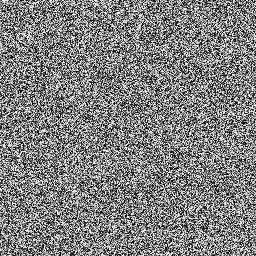
\includegraphics[width=\textwidth]{../images/snowfall.png}
            \subcaption{An image with no nearby pixel similarity, such as this image made up of random numbers, is assumed to never occur among real-world images.}
            \label{fig:snowfall}
        \end{minipage}
        \hspace{0.5cm}
        \begin{minipage}[b]{0.45\linewidth}
            \centering
            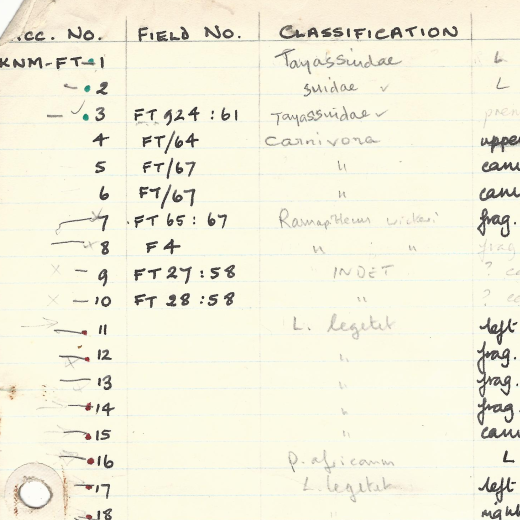
\includegraphics[width=\textwidth]{../images/cataloguesample.png}
            \subcaption{In a real image, most pixel colors are almost equal to neighboring pixel values. Segment from 
            the Fort Tenan Catalogue of the National Museum of Kenya.}
            \label{fig:snowfall2}
        \end{minipage}
    }

        \vspace{0.5cm}

    \resizebox{0.6\linewidth}{!}{%
        \begin{minipage}[b]{0.45\linewidth}
            \centering
            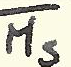
\includegraphics[width=\textwidth]{../images/molar.png}
            \subcaption{Transform invariance: the original tooth notation sample...}
            \label{fig:snowfall3}
        \end{minipage}
        \hspace{0.5cm}
        \begin{minipage}[b]{0.45\linewidth}
            \centering
            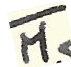
\includegraphics[width=\textwidth]{../images/rotated_molar.png}
            \subcaption{... still keeps its meaning of lower third molar after a transform}
            \label{fig:snowfall4}
        \end{minipage}
    }

    \caption{Visualization of the similarity and transform invariance assumptions encoded in the convolutional layer computation.}
    \label{fig:conv_assumptions}
\end{figure}

%the basic convolution
% convolution (cross-correlation)
% you have input and kernel. input: image matrix (2d) kernel: 2n+1 sized matrix (uneven to make it center around the input pixel processed)
% kernel slides like a sliding window through the input. for each middle position of the kernel:
% result is the dot product of the pixels in equal positions, eq 10.6
% if the image is rgb, kernel is 3d with depth 3. (bike fig 10.10 here)
The layer output computation on a convolutional layer is similar to the fully connected layer computation
presented in Equation~\cite{eq:fc_layer}, but takes as input only a small region around each pixel instead of 
the whole input, and uses same weight parameters on all input positions. To achieve this, the weights of the 
layer only consist of a kernel, a small 
matrix of weights with uneven-numbered size in both the width and height dimensions~\cite{princebook}. During the computation, the kernel 
acts as a sliding window, moving through every possible position on the input image. For each kernel position, an output 
value is produced by computing the dot product between the kernel and the kernel-sized input region around the processed position, and as usual, a bias term is added and the result is passed through the nonlinear activation function.
An example of this basic convolution operation on a grayscale image with kernel size 3x3 is given in Equation~\cite{eq:convolution}. 
For a colored image with three color channels, the kernel becomes three-dimensional. An illustration 
of such case is found in Figure~\ref{image:3dkernel}.

\begin{align}
    h_{ij} = a \left[ \beta + \sum_{m=1}^{3} \sum_{n=1}^{3} \omega_{mn} x_{i+m-2, j+n-2} \right],
    \label{eq:convolution}
\end{align}

\begin{figure}[h]
    \centering
    \includegraphics*[scale=0.4]{../images/3dkernel.png}
    \caption{An illustration of a convolution computation in the case of a color image, from~\cite{princebook}.}
    \label{image:3dkernel}
\end{figure}

% % variants of the convolution: design decisions
% aspects: borders, channels, convolution size, dilation and stride
% default variant reduces size because border pixels cannot be used
% to combat that:
% zero or reflective, padding to keep output and input sizes equal, or valid convolution: dont compute positions where there are not enough previous inputs to use the whole kernel
% channels: run many convolutions in parallel -> more convolution kernel weights to learn
% size stride and dilation, figure 10.3
% size = kernel size
% stride = step between kernel computation
% dilation = kernel is interleaved with zeros, large region but less weights
% stride dilation size fig here
In implementing a convolutional layer, a few design decisions need to be made: how to handle border 
pixels, choosing a channel count, and the shape of the convolution kernel~\cite{princebook}.
For the bordering pixels, where some kernel pixels fall outside of the 
input matrix, the options are to skip these computations, pad the input with zeros, or to pad the input 
by mirroring bordering pixels, the main difference of these being that not padding the input creates a 
result smaller than the input matrix. For the channel count, it has been found that sometimes 
running multiple convolutions side by side creates better results, and the optimal choice of channel count is 
application-dependent. The resulting channels are much like the familiar red, green and blue in an image, but do not 
have any human-decipherable meaning. Lastly, considering the kernel, three aspects need to be chosen: size, stride and dilation.
Size refers to, intuitively, the height and width of the kernel. The stride, commonly 1, controls by how many pixels the 
kernel is slid forward after each activation computation shown in Equation~\cite{eq:convolution}. With dilation, the kernel itself 
is sparse: the weights are interleaved with a desired count of zeros. This allows for larger kernels without increasing parameter counts~\cite{princebook}.

% % pooling
% usually conv layer followed by pooling layer
% pooling
% usually networks are constructed so that  layer by layer layer width decreases and has more depth (more channels, like red green and blue but not with this meaning)
% changing size more than by the few pixels present at image edges: max pooling. take maximum of 2x2 area, collect these values as the output activations. other, less popular variants: mean and average pooling
Usually, a convolutional layer is followed by a pooling layer. The pooling layer adds more nonlinearity to the network, 
and allows halving the layer size. The most common operation is the max pooling operation, where each output pixel is the maximum of
a 2x2 are in the input. Other, less popular operations include the mean and average pooling operations, where the output naturally 
is the mean and average of the small area, respectively. These operations allow for the common structure of convolutional networks, 
where the layer width and height progressively decrease as the computation proceeds~\cite{princebook}.

% relevant here: present the ImageNet competition that has initiated many new architectures.
% % history bit: imageNet breakthrough models alexnet, googlelenet, vgg
% the what models. most influential
% historical scetch: alexnet~\cite{alexnet} brought this to mainstream in 2012, imagenet 2014 saw GoogleLeNet~\cite{googlelenet} and VGG~\cite{vgg}.
% these highlighted because the architectures are utilized in handwritten character classification.
Many advances in convolutional networks have been motivated by the ImageNet image classification competition~\cite{imagenet},
 that ranks models by their capacity of classifying images retrieved from the web to 1,000 distinct classes.
 The results are presented as top-1 and top-5 error rates, the percentage of samples 
where the correct class is not among the one or five most likely classes according to the network. Convolutional architectures
that have performed well in the competition have been found valuable in handwritten character classification, thus the 
breakthrough models presented next are experimented with in later parts of this work.
These most influential convolutional models in the history of the ImageNet challenge,  that
only rely on the basic convolution operation, are AlexNet~\cite{alexnet}, 
the VGG model family~\cite{vgg}, and
the Inception architecture used in GoogLeNet~\cite{googlelenet}.

% alexnet, top5 error: 17\% best so far
% whats new regularization with dropout, large model, large conv kernels (11x11-3x3 kernels), 
% relu instead of previously popular tanhs sped up training, multiple GPUs used when training,
% normalization of convolution results, overlapping pooling (areas of pooling for each pixel overlap)
% impact: brought deep learning to center of ml research, deep nets seem to outperform humans in feature engineering.
The AlexNet convolutional neural network is perhaps the most influential deep learning model of all time, 
popularizing deep learning as a superior feature extractor compared to human-performed feature engineering (ref?).
% what was different
The breakthrough was achieved mainly by speeding up the training process by utilizing graphical processing units (GPU)
in training, a novel idea at the time, and simplifying the feed forward computation by replacing the previously popular 
hyperbolic tangent activation with the ReLU function (Equation~\ref{eq:relu})~\cite{alexnet}.
 This allowed training a larger, deeper network
with convolutional kernels up to the size 11x11, leading to nearly halving the best top-5 error rate with the score of
17,0\%. Other, more minor but still highly influential innovations were the normalization of convolution results, 
overlap in the pooling areas, and using dropout regularization, a regularization heuristic where connections are 
randomly dropped to avoid over-reliance on certain connections~\cite{dropout}.

% googlelenet~\cite{googlelenet} won 2014 with top 5 error rate  6,75\%.
% method: fixed number of allowed multiple-adds in forward pass, 
% used inception (named after we need to go deeper meme) layer: 1x1 3x3 and 5x5 s, also 
% sparse fully connected layers ie not all weights are connected.
% dimension reduction with 1x1 kernels
% to save compute. Also inspired by biological visual systems. allowed
% for deeper and wider network, turned out to be great in imagenet and 
% object detection.
The ImageNet competition of 2014 saw the next breakthrough innovation with the winning architecture of the GoogLeNet,
introducing the idea that smaller convolutional kernels with highly optimized training computation allows deeper,
and therefore more capable networks~\cite{googlelenet}. The layer architecture, named Inception after the 'We 
need to go deeper' internet meme (see Figure~\ref{image:meme}), only used kernels of size 3x3 and 5x5, and
employed dimension reduction with 1x1 convolutional kernels. They also introduced sparsity by omitting connections on 
dense layers inspired by knowledge on the structure of biological visual systems. While these ideas were motivated
by performance-related reasons, the main aim of the study being to fix multiple-add operations available for training 
and to reach as high accuracy as possible, the resulting model ended up reaching a new best top-5\% error rate of 6,75\%
in ImageNet classification.
% sitten spesifiä. 3x3, 5x5 kernels only 1x1 kernels usage in dimension reduction, sparse dense layers to imitate human visual system

% vgg~\cite{vgg}. achieved 6,8\% with imagenet 2014 postsubmission, submitted 7,3\% thus 
% second in competition. method: simple 3x3 convolutions, tested different depths. best depth 19.
% new that previous best models did big kernels and shallower nets. also good model because of 
% the simplicity + the paper included in appendix that demonstrated vgg as a feature extractor to 
% be used in transfer learning.
A close runner-up in the 2014 competition, the VGG model family again proved that deep networks 
with smaller kernels tend to outperform shallow, larger-kernel approaches~\cite{vgg}. The approach 
of the experiments was to fix all kernels to 3x3 size, and to benchmark classification accuracy between 
different model depths. The deepest model with 19 layers was found to be most accurate, and additionally 
to be highly competitive as a feature extractor: an appendix of experiments reached new-best results on a variety of 
further classification tasks. While the 
best top-5 accuracy of 7,3\% ended up with a second place in the ImageNet 2014 competition, the structural simplicity
and diverse learning capacity of the VGG models had a major influence on later deep learning research.

The architectures of the AlexNet, GoogLeNet and VGG models are summarized in Figure~\ref{image:famouscnns}.

\begin{figure}[h]
    \centering
    \includegraphics*[scale=0.2]{../images/ebd.png}
    \caption{The meme that inspired the Inception architecture in GoogLeNet~\cite{googlelenet}, from~\cite{we_need_to_go_deeper}.}
    \label{image:meme}
\end{figure}

\begin{figure}[h]
    \centering
    \includegraphics*[scale=0.6]{../images/famouscnns.png}
    \caption{Architectures of AlexNet~\cite{alexnet}, GoogLeNet~\cite{googlelenet}, and VGG-16~\cite{vgg}, the 
    VGG model variant with 16 layers, from~\cite{zhangImagebasedMethodsDietary2023}.}
    \label{image:famouscnns}
\end{figure}

\subsubsection{Residual connections}

% there was the inspo that it might be that being better at approximating arbitrary functions ie 
% building accurate nns for anything would just be about stacking layers 
% the vanishing exploding gradients problem
%     update a weight parameter w lr*gradient, if gradient is huge you shift parameter a lot, numerically unstable training. if gradient goes to zero, the weight can no longer change 
%     this was already solved with input and batch normalization layers: gradients dont get stuck to some specific values
% another problem: degradation of accuracy
%     deepen deepen the network -> peak accuracy then it reduces
%         so there is something dysfunctional about the standard computation that makes training deep hard 
After the success of the very deep networks (VGG)~\cite{vgg}, the question arised of whether 
achieving better approximation capacity with a neural network simply was about stacking more layers~\cite{resnet}.
The previous major problem of vanishing and exploding gradients had largely been solved by input and between-layer 
normalization operations. The vanising gradient problem refers to when the gradient of the loss with respect to 
some parameters becomes zero, these parameters can no longer be updated with the weight update rule presented in 
Algorithm~\cite{alg:net_training} on line 9 for the duration of the entire training process. Exploding 
gradients, on the other hand, lead to numerical instability as adding a very large number to the weight is 
generally undesirable; the optimum is best approached gradually. Normalization solves these problems by 
updating the activations to a consistent distribution, thus avoiding gradients getting stuck to very large or very small values~\cite{batchnorm}.
However, after stacking even more layers with the help of normalization operations, another issue, the degradation 
problem occurred. This refers to the phenomenon where when iteratively training deeper networks, the accuracy 
reaches a peak and then starts degrading quickly~\cite{resnet}. This suggested that there was something dysfunctional in 
the conventional deep network computations that started showing symptoms when a sufficiently deep network was trained.

% solution, he et al
% if you add identity connection (kinda any layer can be used as the output),
% there are shallower subnetworks in the deeper network -> accuracy can never be worse than 
% in the shallower networks.
%     quick formula and figure here
% turned out to be much better than in the shallower networks
%     hypothesized: the deeper the network the harder it is to learn the identity mapping 
%         this is the cause of the degradation problem and bc residual connection solves it, degradation problem vanishes 
% and indeed the resulting network won many competitions including imagenet challenge with a net 8x deeper than previous deepst, the VGG
As a solution to the degradation problem, He et al.~\cite{resnet} presented the residual connections.
The premise was that if you add a skip connection that can pass any layer computation in the network, 
the deeper network contains in itself all the shallower variants, and the resulting accuracy can never 
be worse than in shallower networks. The skip connection was implemented by adding the input to the conventional 
layer computation, thus the layer computation becomes, expressing the layer without skip connection as $F(x)$, 
$F(x) + x$.
Empirical results showed that this solved the degradation issue, and lead to a 
vast improvement to overall accuracy. It was hypothesized that the reason for the degradation problem 
was that the deeper the network is, the harder it is for the network to approximate identity mappings, and when 
the depth passes a certain threshold, this drawback outweighs the added benefit of more layers. As the skip 
connection makes approximating the identity mapping very easy, all weights in the nonlinear computation can 
be set to zero, the identity mapping problem is completely eliminated. The end results were impressive: 
the ResNet architecture won multiple image detection and segmentation competitions, including the ImageNet challenge 
of 2015, where the new best top-5 error of 3,57\% was reached with a network eight times deeper than the deepest VGG architecture~\cite{resnet}.

\subsubsection{Autoencoders}

% most of this from~\cite{goodfellow}
% labeling costs -> unsupervised learning
% 1. labeling cost eli unsupervised or selfsupervised, which is learning without any labels. x is input and output is latent variable of x, z. if input is an image z is obtained from x somehow eg add noise to image, add 1 to all intensity values, etc. no matter if it makes sense just that there is an algo for getting the latent variable.
As one of the main ways for improving neural network accuracies is to obtain larger training data 
sets, various methods have been developed to increase dataset sizes without adding more manual labeling 
effort, which significantly constraints available data sizes. As the best way to increase dataset 
size without adding labeling effort is to not use labels at all, unsupervised deep learning has been proposed 
as a solution. In unsupervised or self-supervised learning, the desired output for the network to learn is 
derived from the input with a deterministic algorithm. This output is called a \textit{latent variable}~\cite{goodfellow}.
Latent variables can be obtained, for example in the image case, by hiding part of the image given to the input 
and using the whole input as the desired output, or by adding noise to the input~\cite{princebook}.
Due to the nonlinearities in neural network computations, learning the latent variable 
based on the input remains a nontrivial task for the model.

% what is an autoencoder
% 2. autoencoder=input x latent is also x.
% 	normal net: just copy. eg shallow network no hidden units: output at poistion i is input at position j, no learning
% 	trick: constrain
% 		variants: less hidden units than input (undercomplete autoencoders), regularizing encourages smaller parameters or sparsity
% 	most basic: input to hidden (encoder) hidden to input (decoder)
Autoencoders are neural networks trained in an unsupervised manner to learn the identity function: the latent 
variable is the same as the input. To avoid situations where the network would simply copy the values from 
the input layer to the output, the network is constrained. The most common way for this is to use an undercomplete
autoencoder, that has hidden layer sizes smaller than the input, forcing the network to find a way to distill 
the input data so that as much of the original is recoverable on the output layer.
Another way of constraining the model is to add regularization parameters to the 
loss function, encouraging for instance small-valued or sparse parameters as more 
ideal than the trivial solution.
		
% 3. why this is useful / interesting?
% introduce probs the architecture, x h x here
% encoder and decoder nets are mini nets in a net that you take out and use for interesting things.
% - dimensionality reduction/feature engineering by getting the hidden unit
% 	- use features also in character recognition: eg shoponbangla
The natural follow-up question to ask on autoencoders is why bother; what the utility 
of learning identity functions is. For the undercomplete autoencoder, the computation 
can be seen as a mapping from the input to a compressed representation $h$, and 
another computation from $h$ to the input, thus an autoencoder is a mapping $x\to h\to x$~\cite{goodfellow}.
The utility lies in this hidden unit $h$ and that one can take out only the 
computation from $x$ to $h$, called the \textit{encoder}, or from $h$ to $x$, the \textit{decoder}.
The decoder, when trained for generative tasks, can be utilized as a data generator by giving a seed 
sequence as the input.
From the perspective of image classification, the encoder is more useful as it serves 
as a powerful feature extractor: one approach for creating a character-recognizing model 
is to first train an autoencoder and then train a classifier by appending 
fully connected layers to the encoder. This approach has been successfully implemented for the Bangla language~\cite{6shoponBangla}.
Thus, autoencoders can be used as the source 
task in transfer learning, as discussed in Section~\ref{sect:transfer_learning}.

\subsubsection{Transformers and the multi-head self-attention}

% 1 paragraph: motivation for a new method
% nn motivation for a new thing is needed
% words reference to one another that are sometimes far far away in the sequence, conv pays attention only close up with the filter, what is relevant depends on a this word b the other word
% large embedding vectors -> fc layer won't do really, you have to share parameters
The multi-head self-attention layer present in transformer architectures was
originally motivated by natural language processing tasks, as other architectures
encode prior knowledge on language poorly. Words in sentences sometimes refer to 
other words very far from each other in the sentence, which is impossible to model with a 
convolutional layer that only uses the immediate neighborhood as the input for activation computations.
As sequences are processed as splitting the sequence to tokens, for instance words, and generating 
longer embedding descriptors for describing the tokens and their position in the sequence, input sizes become insurmountably large 
to be processed with fully connected layers~\cite{princebook}.

%  2 paragraph: search engine analogue for attention
% embed again a prior by embedding how words relating to each other works.
% search engine analogue.
% query is what we want to find out in the sequence (search query)
% key is a descriptor of the thing (page content for a simple engine)
% value is the search result (page contents ranked)
To construct the self-attention operation, the nature of language was studied 
as an information retrieval problem. The activation value for each input token should be computed 
using relevant parts of the rest of the input, thus one needs a method for ranking the other tokens 
in the sequence by relevance from the perspective of the input token. Using a search engine as an analogue, 
the token can be seen as a query, the input given to a search engine prompt. The alternatives to rank, 
web pages in the search engine case, are the other tokens. The end result, called the value, are the 
available web pages in the search engine case or tokens in the transformer case, ranked according to relevance.

% 3 'the search engine within a phrase' -> dot product self attention
% similarity can be computed with cosine similarity that measures vector direction difference, vec1 dot prod vec2 divided by magnitude (length) vec1 times magnitude (length)vec 2. 
% (give equation for cosine similarity)
% attention with the text sequence between words so self attention
% transformer the query key and value is all the same because we (a sequence and its parts) are paying attention to ourselves (he same sequence), so same embedding multiplied with key query value weight vectors to get key matrix k query matrix q value matrix v
% so then you have the query the key and the value
% query and key is computed cosine similarity qkt/sqrt(dk), scaling factor not quite cosine similarity but similar (lol). you get attention: how much each word pays attention to other words
% softmax to put all attention values between 0 and 1
% second vec needs transpose to avoid dimension errors (matmul takes col from one row from other and we want col from both
% so you have the original sequence and how much attention each word pays to each word (attention filter). multiply original by attention you get the original weighted by how much attention it is sensible to pay between parts
% so this is one head
To find the relevance ranking, the keys (all tokens or all web pages) and the query (a search prompt or an input token)
need to be compared. A rudimentary search engine implements this by computing a similarity metric:
a single value describing how much of the words on the query appear on each web page. This is computed for token embeddings
between the query and key vectors with the cosine similarity, given in Equation~\cite{eq:cos-similarity}. This similarity metric computes the 
cosine of the angle between two vectors, and scales it by vector magnitudes,
 giving a scalar metric with one denoting perfect similarity and -1 perfect dissimilarity.
 In the self-attention operation, as all activations are computed at once, the queries and keys form matrices $Q$ and $K$. 
 To compute the dot product with matrix multiplication, the other matrix is transposed, and the scaling is 
 sligtly varied from cosine similarity by dividing by the square root of the number of tokens, denoted $d_k$. The 
 result is passed through the softmax function (see Equation~\cite{eq:softmax}), to construct an attention matrix where 
 each element describes how much attention should be paid between each token pair. Finally, to get the end result of 
 tokens ranked by relevance, the token embeddings, forming the value matrix $V$, are multiplied with the attention matrix. To include learnable parameters to the layer, 
 the key, query and value matrices are computed by multiplying 
 the token embedding matrices with parameter matrices $W_k$, $W_ q$ and $W_v$. This forms the dot-product self-attention computation, summarized in Equation~\cite{eq:self-attention}.
 
\begin{align}
    \text{Cosine similarity}(\mathbf{k}, \mathbf{q}) = \frac{\mathbf{k} \cdot \mathbf{q}}{\|\mathbf{k}\| \|\mathbf{q}\|}
    \label{eq:cos-similarity}
\end{align}

\begin{align}
    \text{Self-attention}(\mathbf{X}) &= \text{softmax} \left[ \frac{\mathbf{Q}\mathbf{K}^T }{\sqrt{d_k}} \right] \mathbf{V}, \label{eq:self-attention} \\
    \nonumber\text{where} \quad \mathbf{V} &= \mathbf{X} \mathbf{W}_v, \; \mathbf{K} = \mathbf{X} \mathbf{W}_k \; \text{and} \; \mathbf{Q} = \mathbf{X} \mathbf{W}_q.
\end{align}

% 4 multi head self attention
% to be able to pay attention to multiple things at a time you construct multiple attention filters, so do that many times in parallel -> multi-head self attention
% multihead: divide query and key embeddings by splitting embedding matrix, do many self-attention oeprations on those in parallel, concateneate result
% this is the multihead self attention block. here you go a summarizing figure
% each head can focus on different aspects
With the self-attention operation, one limitation remains: one attention layer is only able to focus on one aspect of the 
input sequence at a time. To allow multiple interpretations, many self-attention operations are run in parallel, which is 
called multi-head self-attention. To not increase computation, the token embeddings are divided across the heads, and the 
results from the value matrix multiplied with the attention matrix are concatenated back together, creating a result of 
equal dimension as the one-head version. The self-attention operation with multiple heads is summarized in Figure~\ref{fig:multi-head-self-attention}.

\begin{figure}[h]
    \centering
    \includegraphics*[scale=0.6]{../images/multiheadattention.png}
    \caption{Multi-head self-attention with two heads, from~\cite{princebook}.}
    \label{fig:multi-head-self-attention}
\end{figure}

% 5 the transformer architecture
% transformer architecture uses this and fc layers like so
% transformer is the first architecture to only utilize the attention mechanism (no other layers but multihead self attention and fc layers)
% transformer has an encoder and decoder part (so is a variant of an autoencoder)
% transformer block: multihead self attention and fc layer, both have batch norm after and both have residual connection
% teach the network to continue sentence with the next word, selfsupervised eg hide last word'
% this model was amazing at what check original paper attention is all you need
% tadaa you get a model that can continue the prompt with valid text, add some features and you have a LLM
The main premise of the transformer architecture~\cite{attention_is_all_you_need} is that the multi-head self-attention 
is the only architecture required to successfully learn nature language processing tasks. The first transformer model,
an autoencoder with both the encoder and decoder parts consisting of transformer blocks with a multi-head self-attention and 
a fully connected layer, both followed by batch normalization and with a residual connection, achieved a new best 
result in machine translation from English to German by a significant margin~\cite{attention_is_all_you_need}.
The most famous application of attention-based models is, however, a model taught to continue a sentence fragment with the next most 
likely character. The chat-style variants of these models, most famous being ChatGPT by OpenAI, has become very well known among the general public and 
has even been speculated to show signs of general artificial intelligence.

% 6. paragraph: vision transformer for image classification
% vision application: divide the image to 16x16 patches, interpret those as "words". a transformer architecture that has as output the class probabilities for imagenet. good results but lots of training because transformer does not encode the vision priors of translation and pointwise function invariance
In computer vision, transformer architectures have been successfully implemented.
The most notable of these is the Vision Transformer (ViT)~\cite{vit}, that achieved a top-1 error rate of
11.45\% on the ImageNet challenge, an impressive result yet less accurate than the best convolutional networks of the time.
Falling behind convolutional networks likely was the result of the transformer architecture lacking prior knowledge on images,
translation and pointwise transformation invariance, leading to larger requirements of data and computational resources 
to reach high accuracies. Still, transformer architectures are actively experimented with in many computer vision tasks, 
including handwritten character classification~\cite{9thuonPalm}.

% end of section, back to why i presented these architectures
% these are building blocks that are used for models that classify images. these can be then used for any image 
% classification task like OCR when you use transfer learning which is presented next.
The layer computation variants presented in this section; convolution, residual connection, encoder-decoder chain and 
the multi-head self attention form the set of alternatives commonly used for image classification. Models built with these mechanisms 
have achieved impressive accuracies on classifying the ImageNet samples according to what can be seen in each image.
To utilize these models in handwritten character recognition, a mechanism for applying this knowledge on a new task is required.
This is called transfer learning and is presented next.

\subsection{Transfer learning}
\label{sect:transfer_learning}

% % introduction
% relation to the coarse level training loop: how to initialize model parameters
% basics: what it is, basic premise: if you start out from a parameter configuration that solves a related 
% task well, there is lesser need to train to solve the new problem~\cite{transferlearning_survey}.
Much of transfer learning is about what happens before one starts the neural network training process 
presented in Section~\ref{sect:training}: starting training with a neural network setup, 
architecture, parameterization and training process configuration already successful at a related task,
is known to result in a better model~\cite{transferlearning_survey}. As an analogue to human learning, teaching a human transcriber
to read fossil specimen markings is much easier if the human being has already learned to read.

% this sect from~\cite{transferlearning_survey}. they initially formalized the problem and uniformized 
% the terminology
% % why transfer learning
% why: save compute (imagenet models vgg lenet alexnet training times 5 days to 3 weeks even when using GPUs~\cite{vgg}) and data labeling (usual constraints in ml model building~\cite{engbook})
% also why: training many parameters on a dataset overfits model to the dataset, so freezing layers prevents overfitting~\cite{googlelenet},
% optimization idea: using pretraining that makes sense, you start from a parameter configuration in a 'basin of attraction'
% of a good minimum~\cite{erhanWhyDoesUnsupervised2010}, ie a place where gradients point toward a good local minimum
%     training is strongly influenced by early examples so pretraining prevents overfitting to the supervised task 
%     get sgd trapped in a parameter space that is better so resulst is better even when target data is abundant~\cite{erhanWhyDoesUnsupervised2010}   
% seeing model as model doing the feature engineering: all but last layer are like 
% feature extraction that allows a linear model to be fit from features to output.
%     first layers learn lower level features, higher up more high level~\cite{erhanWhyDoesUnsupervised2010}, so how much to freeze is about how
%     high level features are usable     
% central idea in all of these: model first n-1 layers is a feature extractor

% order of ideas
% sensitivity to early examples
% therefore start with generalist pairs to start -> good basin of sgd -> prevent overfit
% intuitively model has seen more -> better generalization
% practically how done: feature hierarchy is a thing -> freeze first layers
% end result of this
% save compute 
% save labels

Transfer learning has the significant benefits in building accurate neural networks 
of aiding in optimization, generalization and regularization, and saving computational resources and labeling effort~\cite{erhanWhyDoesUnsupervised2010, transferlearning_survey}.
The experimental section presented by Erhan et al.~\cite{erhanWhyDoesUnsupervised2010} found a theoretical explanation for these benefits: they
experimented with ordering of the training data, and found 
that early examples have a significant influence on the further learning trajectory, trapping the optimizer in a parameter region that is later very hard, 
if not impossible, to escape. For this reason, withholding training examples from the actual task until later helps the model not overfitting to the training 
set, as the initial examples do not trap the optimizer to an undesirable parameter region. Intuitively, as the model in this way 
also sees more versatile examples related to the problem, it is known that the end result generalizes better to unseen test data~\cite{transferlearning_survey}.
The practical implementation of transfer learning is better understood when one views a neural network as a hierachical feature extractor:
the first layers learn very low-level features of the input, and downstream layers combine this information to learn higher-level concepts.
In the letter-recognition case, a low-level feature could be noticing edges, and a higher-level feature that the edges curve and intersect in 
specific ways. The idea is that the lower level features are common between tasks, and therefore it is beneficial to reuse them by only 
adjusting the lower layer parameters during training. This approach of not training first layers is also called 'freezing' layers.
By freezing parameters the search space for optimal configuration of the remaining parameters is greatly reduced, saving both computational 
and training data quantity requirements significantly. As data labeling is one of the most laborious aspects of creating deep networks~\cite{engbook},
this is a significant benefit. However, even in cases where labeled training data is abundant, pre-training on another dataset has 
benefits, likely due to the generalization and early example influence aspects discussed above~\cite{erhanWhyDoesUnsupervised2010}.

% % types of transfer learning, terminology
% source task (what y is learned with what x), target task. source/target domain (what X what y)
% inductive transfer, transductive transfer, instance transfer, relational knowledge transfer
% instance transfer: reuse source data
% domain (transductive) transfer (only data differs)
% task (inductive) transfer: tasks differ, data same or different
% task transfer relatedness + the more related the better results
%     negative transfer ie things made worse if things differ too much.
%     super important to consider the distance of transfer ie how similar the tasks are
% broad methods for inductive transfer: feature representation transfer, parameter transfer; priors or hyperparameters of model are assumed to be shared,
% skipped: instance transfer relational-knowledge-transfer: when data is not i.i.d (not considered here)
While the principle of transfer learning was known with many variants and names before, the first survey on 
the topic~\cite{transferlearning_survey} collected all these ideas under the term transfer learning and established further 
terminology related to the paradigm. The first problem solved by the neural network is called the source;
the mapping $X\to y$ is termed the \textit{source task}, and the input and output pair distribution $P(y|X)$ is termed the \textit{source domain}.
Similarly, the next task solved is called the target, with mapping being the \textit{target task} and the data distribution the \textit{target domain}.
A less rigorously defined term for referring to the similarity of the source and the target is in many works called \textit{transfer distance}, and will also be used in 
this work. The subtypes of transfer learning are distinguished by which aspects of 
the source and the target differ from each other, and by how much. The case where the 
source and target task are different is called \textit{inductive transfer}, 
irrespective of if the domains differ. If tasks are the same, but the source and target 
domain differ, \textit{transductive transfer} is conducted. Within inductive transfer, 
re-using parameters obtained by training the source task is called \textit{feature representation transfer},
a common approach. Re-using training hyperparameters is called \textit{parameter transfer}.
Other terms, not relevant for this work include \textit{instance transfer}, where source domain data 
is re-used in target training, and \textit{relational knowledge transfer}, where source and target 
domain are related in a systematic way.

% % using the terminology from  transfer learning, define my problem
% my task. source task is image classification with different data than mine
% inductive transfer where data and task differ.
% i will test both only feature representation transfer (re-search for optimal hyperparameters)
% and parameter transfer (use hyperparameters used in source model training)
% different countries mark tooth fossil in different notation, so fine-tune to adjust
Using the terminology of transfer learning, the problem of reading handwritten 
tooth notation can be formalized in the following way. The source task is image classification,
either of handwritten characters or of images of various objects; the ImageNet task~\cite{imagenet}.
Which one of these works better will depend on for which one the transfer distance is shorter.
This is not entirely obvious in favor of handwriting datasets as they are idealistic benchmark datasets, 
so they might differ from real world character images more than real-world images of other objects. The target task is detecting the tooth markings from tooth character images, and as the source and target 
tasks and domains differ, this is a problem of inductive transfer. The experiments are 
set up in a way that initially, the hyperparameters and 
parameters used in source task are re-used, thus both feature representation and parameter 
transfer is conducted. After that, a hyperparameter optimizer is run, thus the next experiments 
become only feature representation transfer. Should one in the future want to use the model 
developed in this work for catalogues from different institutions, it would be a good idea to 
further train the model on catalogues from the new archives. This would be transductive transfer learning, 
and as the only difference would be a different target domain, the transfer distance is much smaller 
than in these experiments.

% % how transfer learning is used in this work: skip anything that does not do transfer learning
% basically nowadays it is usually insensible to ever train from scratch~\cite{cs231n_transfer_learning}
% therefore this work definitely transfer learns. also previous work that does not transfer learn is dismissed, 
% as it does not inform this case where target data is scarce
In the literature review and experiments presented above, it is assumed that training 
from scratch, starting training from a random parameter initialization, in no case works 
better than transfer learning, a consensus largely shared among the machine learning community~\cite{cs231n_transfer_learning}.
For this reason, research works implementing new character set recognition by training from scratch 
are omitted from the literature search. Only very few articles were dismissed for this reason.

\subsubsection{Foundation models}

% % why
% opening... kinda how far can we take this transfer thing, how far
% Idea: since transfer learning source task performance is not important, target task is the main point~\cite{transferlearning_survey}, 
% you can come up with some nonsensical task such as map image to the same image to get unsupervised task, train 
% massively on massive compute, and use the model for varieties of tasks. idea: do as little as possible in the target domain
% because labeling is the expensive thing~\cite{engbook}, this helps because unsupervised or selfsupervised allows 
% however many labeled samples one wants.
% % what
% come up with task with no value in itself but learns useful features. eg identity mapping in autoencoders,
% mask a part of an image and fill it in, get in a pair of images and say whether they are a transformation of one another.
% save the pretrained model, can be used with transfer learning in manymany tasks
% foundation because foundational traits are learned of the input data
% benefit: regularization
Foundation models can be viewed as an extreme version of transfer learning: how far one can 
move in terms of transfer distance, and how versatilely one can use a single pre-trained model, 
while still reaching adequate target task results. Additionally, as the source task 
performance is irrelevant from the view of the target task~\cite{transferlearning_survey}, one can construct source tasks 
that have no practical value in themselves but are favorable in that obtaining labeled data 
is easy. This is the motivation behind unsupervised and self-supervised pretraining,
tasks where the input-output pairs for the source task can be constructed automatically, and having the 
neural network learn a mapping behind them results in good features. These tasks include the identity 
mapping $X\to X$ of autoencoders, masking parts of the image and having the model learn to
impaint the missing part, or learning which image pairs are transformed, for instance rotated,
versions of one another. Very large models trained with lots of computational resources 
and then used versatilely are called \textit{foundation models}, as they are thought of 
encoding foundational, generic knowledge of the data domain. A famous example of 
a foundational model is the GPT model family by OpenAI, trained 
by giving the model starts of sentences to continue. 
Anyone can test transferring the foundational knowledge on text by prompting the open chat variant of the model a new task, 
such as solving elementary math equations.

% % ocr
% well this is used in ocr as well.
% so you would take some model trained on a large mass of data and then fine tune it on the characters
In handwritten character recognition, unsupervised pretraining is in some cases used 
with autoencoders: the model is trained to reconstruct the input image, and these encoder parameters
are then used in the target task of classifying the images to characters~\cite{6shoponBangla}.
However, this is an approach less established than the supervised pretraining variant.

% end of section
% this section presented relevant background on neural networks
% what you should remember from this chapter
% you have a network that can approximate any input to output mapping
% the network structure is set up in a way that is known to result in a good approximation
% convolution is good with images, self-attention with text but also images, autoencoders 
% with learning the identity mapping
% training is conducted by constructing output from input with the network
% computing difference of output and correct output with the loss function,
% and adjusting the network to a direction that reduces this difference.
% transfer learning means that you start this process from a network state
% that can map some related mapping well, so the optimal network for the new 
% state is closer.
% how to do this in the image to dental element describing phrase case is our topic
This chapter presented background on neural network training relevant for the task 
of classifying handwritten digits. The coarse principles to remember for the following chapters 
are that a neural network essentially is a function approximator. The different structures are 
used to aid in this approximation by encoding prior knowledge; the convolution operation encodes these 
for images, the self-attention for text sequences. Autoencoders are used to conduct unsupervised
learning, where output equals the input. Neural network training refers to finding the best 
parameters to approximate the given mapping, and is conducted iteratively by creating 
an output, comparing it with the correct output, and adjusting the parameters in the direction 
of better output producing parameters. Transfer learning means that this process is started with a 
 parameters that is assumed to be closer to the best parametrization than an average 
random initialization. The following chapters will review previous experiments implementing 
neural network training with transfer learning to solve the mapping task of outputting correct character 
given the image of the character, and experiment with the approaches used the previous successful 
attempts to correctly classify handwritten tooth fossil markings.

\section{Related work}

% intro
% this chapter presents related work from two angles
% angle 1: neural nets & transfer learning on similar problems
% angle 2: solutions to digitization of historical documents

This chapter presents related work from two viewpoints. First, in Section~\ref{sect:related_same_problem},
work on digitizing handwritten fossil catalogues is reviewed. As the work 
in this area is highly limited, Section~\ref{sect:same_solution} presents work using similar techniques 
to ones used here: publications aiming to recognize individual handwritten characters 
with deep neural networks and transfer learning with limited target domain data.

% Search strategy: few seed papers and snowball search. Related conferences: 
% Frontiers in Handwriting Recognition

The literature search was conducted with a snowball search, proceeding with relevant forward and backward citations 
of a few key articles. Additionally, approximately last five to ten years of conference proceedings most relevant for this problem area were 
scanned. For related work on fossil digitization, any found work touching on the subject area will be commented on due to their 
limited amount. For work conducting a similar analysis of handwritten character recognition, more strict conditions were placed. 
For results, to be considered, the work had to be explicit about the best accuracy score achieved,
mentioning the size of the training dataset, number of characters within the classification problem, and the percentage 
of correct inferences with the test set. The source of the base model had to be given along with its source task, training data
and network architecture. The exact method of conducting the model fine-tuning had to be explicit enough to be reproducable,
work simply stating they used transfer learning or leaving gaps in the training process were omitted. Additionally, 
publication venue reputation and acceptable text and presentation quality were taken into account, and some work had to be
omitted because of undecipherable method descriptions or a lack of necessary detail.

% lists best accuracy clearly (percent, which dataset, number of classes)
% specifies the base model used (architecture and source domain dataset)
% specifies how transfer learning was conducted (not just used transfer learning)
% then reputable venue and acceptable quality of text and presentation,
%super subpar text was a frequent reason to skip a paper, they also often lacked relevant details

\subsection{Approaches to digitization of handwritten fossil catalogues}
\label{sect:related_same_problem}

% opening: the obvious solution: sit down and type is pretty much what is done now
While digitizing handwritten fossil catalogues holds,
should all state of the art optical character recognition and data management methods 
be in full use for solving the problem, perhaps a dramatic potential for improving 
the quality of paleoecological research, surprisingly little has as of now been done in this area.
Likely due to the simple fact that the problem has attracted little attention, 
most current work assumes the most rudimentary method: a human 
being sitting down, and transcribing.

%~\cite{uhenCardCatalogsComputers2013} reviews various digital paleo data portals. encourages further digitization but 
% does not really mention how one should go about doing that
%~\cite{mallisonDigitizingMethodsPaleontology2011} review of digitizing fossil data. only considers digitizing 
% physical bone pieces to various 3d images. does not take any stand on digitizing handwritten notes on the samples 
Due to large amounts of transcription work already done, digital repositories of fossil data do exist. A notable review 
by Uhen et al.~\cite{uhenCardCatalogsComputers2013} reviews such databases and encourages further 
digitization of unpublished data, but does not take a stand on how one should complete such work.
Another more extensive review, a whole chapter on digitization methods in paleontology has been written~\cite{mallisonDigitizingMethodsPaleontology2011},
but the chapter exclusively considers digitizing physical bone and plant pieces with various 3D imaging methods, and briefly touches on preferring digital journals over 
paper-printed distribution of research.

%~\cite{groomImprovedStandardizationTranscribed2019} does identify my problem here: most fossil data is in handwritten paper 
% format with many things already known such as taxon. gives suggestions on data format and management but mostly assuming 
% that there is a human transcriber. presents ocr reading as a possibly one day possible option. Notes that especially cleaning of automated ocr read data is a hard problem.
For actual, automated handwriting recognition, a few mentions do exist in previous work. The data management themed 
article by Groom et al.~\cite{groomImprovedStandardizationTranscribed2019} does identify the primary 
problem of this thesis: the article mentions the fact that most fossil data exists as handwritten records with sufficient information 
to conduct analysis without the physical sample, and a big advancement in data availability would be to efficiently and in a consistent 
manner convert this data to a structured database. Optical character recognition is presented, but more as a futuristic option 
not feasible with current methods, and any data quality suggestions implicitly assume that transcription is completed 
by a human being. This review is still relevant for automated digitization as many important considerations in data structuring,
standardization and quality management are presented - revealing the new challenge that should large-scale automated digitization succeed,
the next big line of work would be how to structure and manage the digital paleontological data.

% only work doing the exact same thing:~\cite{shanmugavelHandwrittenOpticalCharacter2018}, but quality of the work is very poor, only 
% presents rudimentary very basic general aspects of image processing such as canny edge detection or contour detection from characters, 
% which is very very far away from working ocr. the paper lists absolutely no results but is an evidence that someone has somewhere at least 
% attempted this.
The only found work solving the exact same challenge as this work is the article by Shanmugavel et al.~\cite{shanmugavelHandwrittenOpticalCharacter2018}.
While the problem is exactly the same, the methods only contain some of the most basic computer 
vision processes, edge and contour detection, and a complete lack of results reveal that not much was achieved in 
this project. However, it serves as a proof that such attempts have taken place in previous years.

% So: to the best of my knowledge there is no other work successfully reading handwritten fossil scans or cleaning 
% already automatically read systems outside of 2024 spring data science project for KNM, for which this is the 
% continuation. therefore also here i will do the simplest things first, since it is a good idea to start with simple and 
% once successful, proceed to harder problems that would digitize and clean more data.
Concluding the review on research articles about digitizing handwritten fossil data, it seems that no successful projects
have as of yet been completed outside of the Data Science student project in spring 2024 for the National 
Museum of Kenya, for which this work is a continuation. For this reason, the experiments in this thesis will 
start out with the simplest problem reductions and only present more advanced techniques as ideas for future work.
The rationale behind this decision is that since not much has yet been done, it is best to start out from 
simple and established implementations to verify simple hypotheses before proceeding to more recently developed mehods.

\subsection{Approaches to handwritten character recognition with small target domain datasets}
\label{sect:same_solution}
% - since there is no old work on fossil i consider other cases and cases that are on abstract level similar
% % 1. PARAGRAPH indian / sanskrit family and why I went for that

% why sanskrit based Indian languages are a good inspo field for KNM

% small languages
% lots of transfer there because languages are small -> small datasets -> transfer needed~\cite{2limbachiyaGujarati}
% major languages have sufficient data to train from scratch (and haven't realized transfer can help even then?~\cite{5rasheedHandwrittenUrduWAlexNet}~\cite{4zhaoTibetan}
% most relevant is how many samples are available per class
% but for knm, asian characters like chinese / korean / kanji could be more applicable because eg kanji contain subcharacter sections (radicals) that have distinct meaning. knm 'radicals': letter number underline. 

% modifiers
% modifiers like knm has the top and low line in: gujarati~\cite{2limbachiyaGujarati} bengali~\cite{3chatterjeeBengali} urdu~\cite{5rasheedHandwrittenUrduWAlexNet}

% cursive~\cite{5rasheedHandwrittenUrduWAlexNet}
% (where it is hard to do connected components based image processing) 

% character sizes vary in bangla~\cite{6shoponBangla}
% also knm with small numbers

% general applicability: bounding box error setting
% also did first bounding boxes (with way easier case tho)-> similar part of character cut off / too much background problems maybe~\cite{1akhlaghiFarsi}~\cite{7rizkybasicCnnTransfer}
% why ancient things could be
% from~\cite{9thuonPalm}
% more than one character per writing unit -> knm also has letter and number
% images + scans are more difficult to read because of old 'paper' -> focus on preprocessing -> similar to knm (but harder than knm probs)
% also pages where you extract characters -> maybe similar ish bounding box extraction mistakes
% huge amount of classes so hardest problem


Due to the limited amount of work on optical character recognition on fossil catalogues, other 
problem domains were chosen to draw inspiration from for constructing the model training setting. 
Interestingly, the nature of the fossil catalogue problem has many aspects in common with reading small, 
regional Indian languages, many of which are based on the Sanskrit language, and with certain historical 
scripts: there are similarities in small training datasets, modifiers, cursive writing and varying character sizes.
While on first thought, languages where a character is a compound of multiple smaller units, such as the 
radicals in Chinese or Korean would be an analogous problem, these are not generally solved with transfer learning 
as the target language has sufficiently large datasets. Therefore, smaller languages such as the south Asian languages studied next with less established public datasets 
are more applicable.
Of these smaller languages, at least
Gujarati~\cite{2limbachiyaGujarati}, Bangla~\cite{3chatterjeeBengali} and Urdu~\cite{5rasheedHandwrittenUrduWAlexNet} all contain modifiers,
which can be seen as analogous to the fossil catalogue under- or overline denoting upper and lower jaw, increasing the problem similarity.
Many characters are cursive in nature~\cite{5rasheedHandwrittenUrduWAlexNet}, which makes especially character segmentation 
solutions more applicable; both the south Asian and fossil catalogue characters are closer to equal in segmentation difficulty.
The last trait making these languages applicable is that character sizes vary in many, at least in Bangla~\cite{6shoponBangla}, which 
is also the case in fossil catalogues with the smaller upper and lower script characters.
For the historical scripts, a study on machine reading historical manuscripts written on palm leaves was 
included in this review as the scanning of these scripts is more challenging due to the old leaves, and thus the 
study contained valuable insight on image quality enhancement techniques~\cite{9thuonPalm}. Additionally, historical scripts 
contain far more characters than modern languages, making the problem more challenging and thus more interesting.

% 2. on quality

Before each of the reviewed articles is presented in more detail, a few points on the overall quality of the work studied must be noted.
 Unfortunately, the analytical basis of the work reviewed was quite lacking; for the most part, model training setup decisions were made 
 without any reasoning for why the decisions were made. Especially lacking are analyses on how similar the source task 
 is to the target task, which would be critically important in getting transfer learning to work properly. 
 Also unusual choices would have been useful to have a reason, but these were mostly missing. 
 Where a reason was given, it often only resorted to listing general strengths of the technique chosen,
  but still lacked the most important part; why this technique was better than other available alternatives for this specific task.

The reasons and considerations regarding setup decisions are not nice-to-haves, 
but have quite some consequences for the quality of the research conclusions. In later work, one cannot evaluate
 the reasoning behind the choices. For some choices, it can be noticed that they do not make much sense at all, an example of this being 
 using image horizontal or vertical flipping as a data augmentation technique for character images~\cite{9thuonPalm}
 (in latin letters for instance, a flipped L could become a J). Also, some test data setups become questionable from a 
 generalization perspective, such as hyperparameter optimizing for the best angle to rotate every image 
 as a data augmentation technique~\cite{7rizkybasicCnnTransfer} (the idea of data augmentation is to augment
  the data set with valid images that just happen to not occur in the test set, 
  and it is hard to imagine a case where only one rotation angle would produce valid training images), 
  or applying data augmentation for the test set~\cite{11zunairUnconventionalWisdom} (when all test images are not real-world samples, 
  test accuracy is not a good representation of real-world performance). 
  Irrelevant specifications are occasionally given, such as hardware when runs are not timed~\cite{9thuonPalm}, and relevant details, 
  such as if parameters were frozen, are sometimes omitted~\cite{8goelGujarati2023}.
  Less relevant metrics are measured, such as inference times even when the model is not part of a real-time system~\cite{8goelGujarati2023},
  or metrics where the exact definition is unclear, such as positive and negative related rates~\cite{10goelGujarati, 5rasheedHandwrittenUrduWAlexNet} when the definition or implications
  of non-class-specific positive/negative related metrics is unclear in OCR in the usual case where correctness is equally important
  among all classes. Finally, analytical comparisons become frayed, such as the statement that a worse accuracy is compensated by the
   benefit of having to train for less epochs~\cite{3chatterjeeBengali}, when training in an OCR transfer learning setting is generally completed in order of minutes even on a CPU.

Due to these limitations of the reviewed work, the unexplored alternatives cannot be crossed out as probably unlikely to work well. Therefore, this work will experiment with some other than the most popular approaches that are implemented in the works presented next.

% 4. incremental recognition of tibetan

% contribution: outperform from scartch single model detects all tibetan by creating styles classifier, training resenet 50 from scratch with tibetan and transferring from that to different styles

% relation to my case: they also need to learn many things: style and what character it is. take the high level approach from here
% 	simplify problem by dividing it so that each model has a single task. This eases need for data samples in quantity + makes collecting them easier

% miscellaneous probably extra info
% base model resnet (only generic reasoning why), two layers added in finetuning
% 	script classifying base model was vgg16 because of robustness
% data is not well balanced
% they saved large amount of compute percentage wise (2/3), but not much in absolute running time (40 minutes)

Zhao et al.~\cite{4zhaoTibetan} achieved new state of the art accuracy in multi-style Tibetan glyph classification
with a model chain approach that first classifies glyphs by style and then recognizes the glyph with a style-specific model. As these downstream
 residual learning models are trained with transfer learning with a Tibetan 
 recognition model as the base model, the source and target data domains are very similar,
  thus the transfer setting is simpler than in the fossil catalogue case. However, the approach of 
  chaining simple classifiers as a solution to a more complex problem served as an inspiration for
   the pipeline approach implemented in this thesis.

% 1. farsi handwritten phone numbers

% what
% image of phone number -> segment to individual digits -> train digit classifier from scratch
% especially chosen because they have this pipeline approach like I do

% good/bad about this paper analysis
% 	much simpler approach
% 		tiny network (only 3 conv layers), no transfer learning, still 99,37% accuracy
% 		finding a smaller architecture + training with domain dataset could result in smaller model (but: more likely to overfit because of no source data, would not work that well with small datasets like KNM). 
% 			but reasoning why people do imagenet transfer is so good it does not necessarily pay off to do this. they did not say how long they searched until they found this architecture. humanity has spent a long time to find best imagenet architecture so maybe rather not reinvent the wheel. also archival digitization inference is never real-time so save energy for other problems that matter (shrinking model size has no real benefits and finding it would be more work so work with no prize)

% this is another work with not entirely identical setting but otherwise inspiring traits: they also did segmentation and then classification so another full pipeline implementation

As another pipeline approach for detecting characters out of a longer sequence, Akhlaghi et al.~\cite{1akhlaghiFarsi} implemented 
a reading system for Farsi phone catalogues by chaining a gradient histogram based segmentation 
algorithm with a digit classifier. While the segmentation task is due to uniform character
 sizes much simpler than the catalogue case, the work has a possibly useful literature review on
  character segmentation. For the classification, a very small convolutional network was trained
   from scratch to a satisfactory accuracy of 94,6\%, proving that with careful architecture design,
    even small models can learn to accurately classify digits.


The rest of the literature reviewed in this section is directly analoguous 
to the fossil case: a ImageNet or autoencoder base model is trained with transfer learning to detect a new set of characters.
% 5. rasheed, handwritten urdu characters

% what 
% urdu digit/character ocr with transfer learning on alexnet.
% svm used, but is outperformed by finetuning

% my approach selection / the why + lack of quality problem
% the paper quality was so low and many details not given

Rasheed et al.~\cite{5rasheedHandwrittenUrduWAlexNet} created an AlexNet-based Urdu recognition 
model, achieving 98,12\% accuracy in digit recognition. The common last layer replacement 
with a fully connected layer with softmax activation was benchmarked against using AlexNet as 
a feature extractor before support vector 
machine classification, the former giving the best result.


% 3. chatterjee bengali handwritten character classification
% what
% 	most (but not all) bengali character classification with finetuned resnet. 
% 	superfancy tinetuning process, aims to converge in small number (48 so not even that small) of epochs, no reason why this is important, why simple ordinary finetuning wont do
% critique on (transfer) method
% 	transfer method is very complex, not quickly decipherable. Point of this seems to optimize for less epochs, which is not really necessary imo. so don’t do this unless simple things take forever (which never happens so don’t do this)
% major WTF
% ”if we remove misclassified data points, accuracy would increase”

For Bangla character classification, Chatterjee et al. reported 96,12\% accuracy 
by fine-tuning a ResNet model. The work employed highly sophisticated transfer
 learning and learning rate scheduling algorithms, aiming to converge training in as 
 little epochs as possible, an aim already discussed to not likely be worth the pursuit.
  Another concern was the concluding statement "if those misclassified points were 
  removed from the dataset, the accuracy will improve further", which was not done 
  to keep the benchmarking accurate.

  % 6. shopon bangla handwritten digit recognition using autoencoder and deep cnn

% what
% autoencoder based outperforms basic cnn things in bangla, new best

In Bangla digit classification, Shopon et al.~\cite{6shoponBangla} implemented unsupervised 
pretraining and found a new best accuracy in Bangla digits
and best accuracy among all articles reviewed in this section of 99,5\% by chaining an autoencoder
with a deep convolutional network. This proves that while less popular, unsupervised pretraining
based approaches are worth experimenting with.

% 11. zunair unconventional wisdom

% contribution: test different transfer approaches w vgg base model for best performance
% best one has much more parameters (more thatn 1000x more) than 'conventional' transfer approach
% first to use transfer on bengali numerals

% critique/quality issues
% freezing intermediate layers does not make sense from the low to high level features perspective... you cannot really freeze layers that have unfrozen layers ahead because later layer is always based on the previous one -> frozen layer computations don't make sense anymore 
% better than "conventional transfer learning" bc less epochs and parameters -> are you assuming conventional transfer is the fine tune whole model approach? that is not correct? if you assume eg train fc layers as conventional then the less epochs/parameters statement is incorrect.
% 	they state that only last layer is trained is the conventional transfer learning approach. then i don't understand how freezing less than this would reduce count of trainable parameters
% lack of understanding: an experimetn where they froze the last layer! it was randomly initialized!
% they are like weeeel! it works! wtfff
% test set augmentation > test setting is not realistic real world data. based on figs also train and test data look very different
% overall presentation/quality not great

Lastly for the Bangla language, Zunair et al.~\cite{11zunairUnconventionalWisdom} experimented 
with very unconventional transfer learning approaches to classify digits.
The authors experiment with freezing layers below not frozen layers, an intuitively odd 
technique as later layer computation is very dependent on the output of the previous ones.
Another even more preculiar approach is to immediately freeze the last fully connected layer, 
hindering any updates to the randomly initialized weights. The end result of 97,09\% is stated 
to prove that these unusual approaches are worth experimenting with further, but due to this 
result being only found with this one data set and one base model, VGG16, and without any 
theoretical basis, the evidence for the sensibility of this approach is not quite sufficient.

% 2. identification of handwritten gujarati alphanumeric

% what
% create gujarati alphanumeric dataset + transfer cnn to build a classifier

Several articles detected characters form the Gujarati language.
Goel et al.~\cite{10goelGujarati} were the first to attempt deep learning for Gujarati digits, 
achieving 96,5\% accuracy with the EfficientNet architecture. However, the authors utilized 
validation error on the test set as a training stopping condition and then reported accuracies 
on the same set, leading to data leakage and a result not necessarily representative of true
generalization capability. In a later article~\cite{8goelGujarati2023}, the authors expanded 
their experimentation to other architectures, created several transfer learning settings informed 
by analysis on source and target task similarity, fixed the data leakage issue, and reported an 
improved accuracy of 97,92\%, again with the EfficientNet architecture. Additionally, adding a fully
connected layer is again found to outperform using a support vector machine as the downstream classifier.
Limbachiya et al.~\cite{2limbachiyaGujarati} implemented digits and letters detection by comparing various convolutional architectures,
 achieving the best accuracy of 97,03\% with the MobileNet architecture. Transfer learning was implemented with a
  less usual top layer architecture: dropout was added between two new fully connected layers.
% 10. goel a prettrained cnn based framework for handwritten gujarati
% what
% test dl + transfer learning for gujarati digit classification (first one to do that)
% whys / quality things
% transfer method is chosen based on transfer distance but transfer method is so
% vaguely described + no code published u cannot know really how it was implemented (training form the starch etc)
% they seem to not understand stuff properly
% data leakage: only train and test sets +
%training stopping condition is according to ’best validation error’ -> apparently no validation set -> training is informed by test error -> data leakage -> accuracy is not generizable

% 8. handwritten gujarati numerals goel

% what
% publish a data set
% test 10 models 3 transfer methods, find how to implement transfer for gujarati (devanagari language from india, maybe sanskrit based idk) digit recognition accuracy
% best paper so far, gives reasons for some (not all!!) decisions, considers transferability
% methods are: feature extractor w svm or fc layer classifier, finetuning half of the base model. basic fc layer approach best of all. tested mnist as base, did not work as well
% also bounding box extraction to get digits with usual smoothing filter then threshold then contour detect method. big problems with discontinuities in characters -> will not work in fossil

% 7. text recognition on images using pretrained cnn, rizky

% contribution: prove that using imagenet weights makes sense (which was kinda known already), surprising result: freezing is worse than not freezing (state on well dataset size was this and this big so maybe thats why). uses benchmark dataset so maybe easier problem than in the wild but dataset that tries to have more ’difficult’ ocr. handwriting and typed
% first: compare models. then: compare freezing layers with the best model

% data leakage/limitations
% hyperparam optimizaton for best rotation angle etc. they have train test val datasets but did not say if they used test set to inform decisions. this smells like fitting to test set: eg range of roatation angle could make generalization sense: images are by this n this much rotated, but always rotated the same angle does not have a sensible interpretation. also they did not spec why they optimized this, they just did it
% test set size on the iit5k dataset is only 30 images (with many characters in each image but still about 150 samples)

% why
% they gave a why for why cnn, but said that its because cnn ’works’. but 2022 and many new methods exist that tend to outperform cnn. what abt them?

As the only work reading characters from a banchmark dataset of handwriting, Rizky et al.~\cite{7rizkybasicCnnTransfer}
first compared various architectures and then used the best model, VGG-16, to compare multiple transfer learning 
approaches, reaching a final accuracy of 98,16\% by fine-tuning the whole network. However, to achieve this accuracy, the exact best data augmentation parameters of 
rotation angle, image scale and blur style are searched for, raising concerns of real-world generalizability of this result.
 While the dataset is likely to be easier than the fossil case, the relative accuracy of 
various approaches can give valuable insight to inform choices in designing the dental marking recognition model.

% 9. palm

% what-contribution
% investigate effect of preprocessing/augmentation/dataset expansion, compare cnn and transformers. do ocr w transformer / cnn in this case - not done before much. big image quality focus, much more than other papers
% cnn better than vit, binary better than gray/rgb (my: interesting: maybe benefit of less meaningless signal outperforms bad side of increasing transfer distance)
% more data and preprocessing works better, pretty obvious. but nothing on if its the preprocessing or the more data that did the trick
% why transformers worse: limited memory high computing requirements (no idea what limited memory means, only remembers recent training instances or whatt)

% why
% why for transformer: has lotsa attention (network effects...)
% why resnet: less complex than vgg

% quality things
% no validation set, possibly data leakage

% misc / maybe dont mention
% some methods they used idk
% dropout
% stochastic depth regularization 

% metadata for summary of papers table / table, how to do paper analyzing

% 7.
% - language + main country where its spoken to see geographical representation of  languages analyzed in the papers
% 9.
% - maybe state number of params for each base model to give a vague sense of how many there are in each
% - directly state which variant of the model was used bc i also need to pick a variant (eg vgg16 or vgg19)

Lastly, a very interesting application case of reading characters used in ancient historical scripts written 
on palm leaves, Thuon et al.~\cite{9thuonPalm} achieved a very impressive accuracy of 93,55\% on more than 100 
classes from challenging palm leaf scan images. The work includes many valuable parts: image enhancement,
data augmentation and dataset expansion insight, and comparison of multiple convolutional and attention based model 
architectures. As the main result it is concluded that convolutional networks tend to outperform transformer architectures.

Details on all the works presented above are summarized on Tables~\cite{tab:dataset-info} and~\cite{tab:model-info}. Where multiple settings 
were experimeted with, the class count producing the highest accuracy score and the three best 
base model variants are listed starting from the best for brevity. The Tibetan detection article~\cite{4zhaoTibetan}
is omitted due to transfer setting being very different to the other works. Replacing the last layer with a 
softmax layer with ouput size equal to target class count is not 
stated in the table as it was done in every case. The shorthand 'FC' is used to denote a fully connected layer.

\begin{table}[h!]
\centering
\resizebox{\textwidth}{!}{
\begin{tabular}{|c|l|c|c|}
\hline
\textbf{Article} & \textbf{Language} & \textbf{Number of Classes} & \textbf{Samples per Class} \\ \hline
\cite{1akhlaghiFarsi}                & Farsi             & 10                         & 8,800                       \\ \hline
\cite{2limbachiyaGujarati}                & Gujarati          & 54                         & 1,400                       \\ \hline
\cite{3chatterjeeBengali}                & Bangla            & 84                         & 1,977                       \\ \hline
\cite{5rasheedHandwrittenUrduWAlexNet}                & Urdu              & 10                         & 840                        \\ \hline
\cite{6shoponBangla}                & Bangla            & 10                         & 2,922                       \\ \hline
\cite{7rizkybasicCnnTransfer}                & English           & 36                         & 2,055                       \\ \hline
\cite{8goelGujarati2023}                & Gujarati          & 10                         & 800                        \\ \hline
\cite{9thuonPalm}                & Ancient Balinese (1), Sundanese (2), Khmer (3) & 100 (1), 111 (2), 60 (3) & 193 (1), 1,836 (2), 122 (3) \\ \hline
\cite{10goelGujarati}               & Gujarati          & 10                         & 250                        \\ \hline
\cite{11zunairUnconventionalWisdom}               & Bangla            & 10                         & ~8,500                     \\ \hline
\end{tabular}
}
\caption{Literature Summary: Datasets}
\label{tab:dataset-info}
\end{table}


\begin{table}[h!]
\centering
\resizebox{\textwidth}{!}{
\begin{tabular}{|c|c|l|l|}
\hline
\textbf{Article} & \textbf{Best Accuracy} & \textbf{Base Model(s)} & \textbf{Transfer Method} \\ \hline
\cite{1akhlaghiFarsi}                & 99.37\%                & New Architecture       & -                        \\ \hline
\cite{2limbachiyaGujarati}                & 97.03\%                & MobileNet, DenseNet, VGG16 & Train new FC layer + dropout + output \\ \hline
\cite{3chatterjeeBengali}                & 96.12\%                & ResNet50               & Train all layers, increase learning rate for later layers \\ \hline
\cite{5rasheedHandwrittenUrduWAlexNet}                & 98.21\%                & AlexNet                & Train all layers but last layer most \\ \hline
\cite{6shoponBangla}                & 99.5\%                 & Autoencoder (trained on Bangla) & Append small deep CNN to autoencoder, no freezing \\ \hline
\cite{7rizkybasicCnnTransfer}                & 98.16\%                & VGG16, DenseNet121, ResNet18 & Train all layers        \\ \hline
\cite{8goelGujarati2023}                & 97.92\%                & EfficientNetV2S, Xception, ResNet101                    & Train all fully connected layers \\ \hline
\cite{9thuonPalm}                & 91.85\%                & EfficientNetB0, EfficientNetB1, ResNet101 & Freeze first layers \\ \hline
\cite{10goelGujarati}               & 96.5\%                 & EfficientNetV2S, InceptionV3, ResNet101 & Add 2 FC layers + output layer, no freezing \\ \hline
\cite{11zunairUnconventionalWisdom}               & 97.09\%                & VGG16                  & Freeze layers 16-20 (3 convolutional, 1 pooling layer) \\ \hline
\end{tabular}
}
\caption{Literature Summary: Accuracy, Base Model and Transfer Method}
\label{tab:model-info}
\end{table}

% summarizing chapter
% what should the reader remember?
This chapter presented work related to the problem of recognizing handwritten dental 
fossil markings. Since little previous work on fossil catalogues existed, the attention 
was turned to a related problem on an abstract level; recognizing handwritten letters
and digits in South Asian languages. The insight gained from the 
literature review will be used in creating the model training setup for the required 
deep learning models.

\section{Experimental setup}

% consider the fossil case again.
% my goal in this work is ...
The goal of this thesis is to recognize tooth type,
jaw and index number markings to increase the accuracy of the element description in
the digitized fossil dataset of the National Museum of Kenya. This 
chapter presents an end-to-end system that achieves this goal and gives reasoning 
for the training setups tested to build  the required deep learning models.

% the hypothesis: pipeline approach of classifying teeth to types with a series of models will result in highly accurate cleaned tooth data
%     verify that this is possible
%     experiment with base models and layer freezing to find best accuracy score
The main hypothesis is that accurately recognizing tooth notation in catalogue images 
is best completed with a divide-and-conquer approach: by decomposing the main problem into small
subproblems of simple univariate classification, and chaining these to a tooth detection pipeline,
the subproblems become easy enough to be solved with perfect accuracy on limited data.
The aim of the experiments is to verify the plausibility of this approach and find the most accurate deep 
learning models to solve the subproblems involved.

% overview of chapter
%     sect 6.1 formulate the problem ie how to interpret the ambiguous goal of 
%     "clean element description tooth markings" set of x to y mappings that can be taught to a deep neural network
%     and how to build a system from the mappings that achieves the goal
%     sect 6.2 the training settings attempted informed by literature
%     for creating the models are chosen
This chapter is organized as follows. In Section~\ref{sect:problem-formulation}, the tooth recognition problem is formulated as a set of $X\to y$ 
mappings that achieve the goal of cleaning dental markings in the element description column.
Then, training settings attempted to build the required models are chosen, informed by literature, in Section~\ref{sect:building-models}.

\subsection{Problem formulation}
\label{sect:problem-formulation}

% point of this section:
% what data we are talking about, what has been done, what is my goal on high level 
% subsections formalize the high level problem to a problem that can be solved with a nn
To give an exact task to a neural network, one needs to explicitly define 
the inputs and outputs to the network, and determine how they will be obtained and used.
 As this work is a continuation of 
a previous digitzation project, this section first presents the starting point 
from the project output and characteristics of the scan images. 

% data and what has been done until now
% what the catalogue is exactly: tabular handwritten log of fossils
% element description column (which part of the animal)
%     handwritten notation from time before standardized computers, so very variable writing with no notation standard
%         -> rare surprise characters occur (eg 1/2 as a one half of a tooth noter)
%             old note on this: has been done by different but few annotators, no logs on who logged what, everyone 
%             had a bit different style of notating. also no clearly defined standard 
%             for notating specimens. so might be that actual data used will have 
%             characters or words not present in training set
% photo-to-tabular has been done but
%     teeth have errors in ocr output (eg tooth types that are not m p i or c)
%     upper lower jaw is unknown since ocr used in table (azure) cannot read up/low jaw notation
The fossil catalogues are hand-drawn tables with specimen details such 
as accession identifiers, localities and element descriptions. The element description 
column specifies which part of the skeleton the fossil is from and therefore is the only 
column with tooth notation.
As no exact standard was required, perhaps because only a few people 
created the markings, there are inconsistencies in notation style. Additionally,
ad-hoc symbols such as fractions are used with only a few occurences in the whole set of catalogues. 
A sample of the catalogues is presented in Figure~\ref{image:cataloguesample}.
The previous project managed to digitize most of the contents of the table, but since 
the generalist Azure Vision model~\cite{azurevision} was used, tooth notation recognition
loses information of upper or lower jaw and sometimes
erroneously recognizes tooth type letters and index numbers.
The aim of the experiments in this work is to fix these errors.

\begin{figure}[h]
    \centering
    \includegraphics*[scale=0.5]{../images/cataloguesample3.png}
    \caption{A sample from the fossil catalogue sheets of the National Museum of Kenya}
    \label{image:cataloguesample}
\end{figure}

% what i am doing now
% with the catalogue is to take an element description (give sample image).
% of this description, i should find what teeth are mentioned, and list them as a tuple 
% in another column. (give what teeth there are) and put the cleaned teeth to 
% the description instead of the not clean word
% to aid in this i have also the generalist OCR ouputs from azure (bounding boxes are assumed)
The aim is to augment the digitized dataset with a tuple of all teeth in the 
element description, and to correct the erroneously read tooth markings in the element column.
The digital notation, presented in Table~\ref{table:jaw_notation}, is used in the end result.
The recognition will be built assuming that bounding boxes for cropping out individual words in the 
catalogues are available; for this purpose, Azure Vision output files with bounding boxes
are used. An example of the desired output,
created by hand-annotating, is presented in Figure~\ref{image:goal}. 
As can be seen from the dataset sample, the other data in the end result is far from perfect, thus
 much remains to be done after this work.

\begin{figure}[h]
    \centering
    \includegraphics*[scale=0.5]{../images/goal.png}
    \caption{The goal: teeth are listed in tooth records column and the description column contains correct markings.}
    \label{image:goal}
\end{figure}

% so: we have the vague goal of catalogue to cleaned element description with teeth tuple extracted.
% general on goal to nn: the generality vs accuracy tradeoff and what i should aim for
% different types of defining inputs and outputs, discussion on what to choose
% generality ease trade off: constrain to simple input output relation causes model to be 
% more accurate (it can be given more prior information on what is present), but less applicable 
% to variability in data.
% example of very constrained setting
%     input: perfect images of teeth letters
%     output: letter
% example of a very unconstrained setting
%     input: the whole catalogue image
%     output: a tabular dataset of all text there perfectly cleaned no matter the anomalies
% why we went for more simple approaches first
%     because the part of data that can be digitized with the tightest constraints and the simplest models are most accurate. Do that first, deal with the remaining later
%     better to clean small subset of data well than large amount of data badly.
%         difference to other domains of big data:
%             each fossil sample is expensive and human laborous to obtain, thus "big" sample is 
%             small compared to other ml applications, 1000 is a lot 10k huge.~\cite{Faith_Lyman_2019}
%             so get a clean sample that is small is still valuable because paleo samples are relatively small
%         also: not much done before so it is better to start out simple and build from there
The guiding trade-off to discuss when choosing the neural networks that could aid in correcting
tooth notation is between accuracy and generality. The more prior information one gives to 
the model, or the more constrained the task is, the better the results are. On the other hand, a too
constrained model is poor at handling the inevitable variability in human-written text.
The implemented approach aims to start from more constrained models for multiple reasons. 
As fossil datasets are a relatively unexplored domain in character recognition, starting out from simple
solutions is reasonable. As one can always filter for and recognize the easiest 
cases, for instance teeth where the segmentation result is best,
simple cases present a low-hanging fruit worth starting out from. As more generalist 
models are usually less accurate on all samples, they make more mistakes even on
easier cases. Additionally, as the aim of automated digitization is to avoid tedious manual verification,
 only models with near-perfect accuracy are usable, since even in a case of minor insecurity the sample needs to be checked.
As sample sizes in paleontological studies are relatively small, the cost of a data mistake
can be severe and is amplified by these errors propagating to every study that uses the data point.

% first question: is the input the whole phrase, words or characters? sect sequence learning. 
% since words are better, section tooth thinks about how to solve image of word to tooth type problem.
% once we know how i show u how to use the models, how the system will work
With the end goal of correcting tooth notation and guiding design principle of starting out simple in mind, the next sections will discuss two major questions 
in how to set up the tooth recognition system: whether to give the whole element desctiption cell content
 or only a word to the model, and how to set up target classes for the classification tasks.

\subsubsection{By-sequence or by-word recognition}

% sequence definition: image to variable-length phrase (text in the image)
% word per word approach, inspired by~\cite{tibetan_ocr}:
%     input is image of one word
%         one tooth = one word
%     output is the text on the image, when the word is a tooth output is valid tooth notation so m1-3 p1-2 etc
% character by character approach: input character image, output character 
%     we cannot do this because there is no readily made segmentation of image to characters 
%     would also not make much sense because tooth notation letter and number should be kept together
%     -> choose between sequence and word
To choose the inputs for models, one needs to choose whether to keep the
element cell contents as one image or split it to words. As the segmentation 
data is only available up to word level, the character option is not available in this work.

% sequence benefits:
%     adaptable to many kinds and lengths of input
%     also clean the nontooth word outputs at the same time

% sequence bad sides:
%     finetuning just one layer on 80 training images for two epochs took about 15 minutes of~\cite{li2021trocr}
%         -> all hyperparameter optimization etc is out of question with this heavy training.
%     finetuning on images with tooth data caused errors on words that 
%         (give a sample of confused reading attempts: leftleftleftleft)
%     inductive transfer learning is the case here, target task differs from source task
%         the target set of characters has changed
%             Encoding this to the large encoder decoder transformers would 
%             require rewriting parts of the preprocessor and model which is too complex given the level of this work.
%                 only adequately accurate models are large collaboration efforts to create so code is complex 
%                 eg trocr is by Microsoft employees
Sequence learning is a machine learning paradigm where both input and output lengths vary~\cite{sutskever2014sequence}.
The clear benefit is its flexibility; more difficult cases such as many teeth noted together (eg. $\text{M}_{1-3}$),
where segmentation to words frequently fails, could be recognized. A fine-tuned sequence learning 
model could also be given prior information on the paleontology domain of the text, making
most of the English vocabulary impossible to occur and therefore constraining the problem. As for downsides, the practical hindrance is 
that flexibility requires huge parameter counts: fine-tuning the 
Microsoft TrOCR model~\cite{li2021trocr} was attempted, but available labeled data and computational 
resources proved insufficient to train the model even when updating only one layer,
and outputs of untuned smaller models on basic handwriting were not satisfactory.
A theoretical description of this is that because both the domain, from general handwriting to fossil catalogues, 
and the task, the character set to recognize, changed, the transfer distance becomes so large 
that significant training data and computational resources are required to teach the new problem to the model.

% word by word benefits
% feasible given available data and computing resources
% possible to encode the tooth type classes, eg have a class "third molar"
% classifying characters has been essentially solved, easy problem 
% also classifying to tooth or not tooth should be easy 

% word by word bad sides
%     not as flexible. but we started with the easier anyway to have something thats working
%     left right cannot be put to tooth markings sometimes in other formats like "left mandibular frag with m1-2"

% so, word by word. next: formulate image of word to correct output more precisely
Recognizing the markings word by word becomes character classification in 
the tooth marking case if one constrains the input images be samples with one letter and 
one number, leaving out the multi-tooth markings with a number interval (eg. $\text{p}_{2-4}$).
This has the benefit that after rather easy binary classification of a word to 
tooth marking to other word, priors on the dental row can be encoded in the classification
task. By having, for instance, one class for each tooth type, count of target classes becomes
relatively small, making the problem solvable even with small amouts of data.
The drawback is a lack of flexibility, propagation of 
bounding box detection errors and that left and right jaw information has to be left out from 
the tooth records column: the jaw side information is not always given in the same word, 
in format such as '$\text{LM}_1$', but in other parts of the description, in formats like
 'left mandibular frag. with $\text{M}_1$'.

Given the problem of classifying a tooth notation image with a type specifying letter and an index 
number, the classification problem is formulated next.

\subsubsection{Tooth marking classification: multi-label classification or classifier chaining}

% approach: tooth or not tooth. then classify teeth. 
% not tooth straightforward: use azure output
% tooth less straightforward, topic here: x is the image of the marking, y is tooth type, but what is the 
% softmaxed probability vector the model should output? so what are the target classes?
Given the choices that processing is completed word by word and leaving more variable inputs like 
notation marking multiple teeth for future work, the output still requires to formalizing.
Processing non-tooth words is straightforward; as the Azure Vision results are accurate, they
can be reused. Less straightforward is which classes to set up for the 
tooth markings: the image has many points of information; tooth type, jaw and index number with 
interdependencies, like the index number range depending on the tooth type.

% formulation of tooth image to tooth type
%     univariate: m1,m2,m3,p1,p2,p3,p4,c,i1,i2,i3 up and low (22 classes)
%         -: does not encode that all m's share letter m, all ups share traits
%         we have kinda three separate problems: 123, updown, mpic. this does not encode that 
%         but states we have one problem with 22 possible, separate solutions with no relations between solutions
%             (all classes are equally dissimilar to each other) --> incorrect encoding of prior knowledge
%     alternative multivariate: up/down, MPIC, 1234
%         input image, output three vectors: updown, mpic, 1234
%             -: multiclass classification general case does not work like this 
%                 general case is like image can have a dog and a cat, but here an image cannot be m and i~\cite{multilabel_classification}
%                     so this is special grouped classification -> less prior work as problem is more unusual 
%             -: no such thing as a 3rd canine 
%                 so not all variable combinations are possible. no easy well established way to encode that to the model 
%                     what will we do if the model thinks its a 4th canine?
%             -: even when it was easy~\cite{tibetan_ocr} kinda already argued the multilabel is a bad approach
The simplest formalization would be to have one class per tooth, the classes becoming for lower jaw m1-m3, p1-p4, c and i1-i3,
totaling 22 classes when including both jaws. This, however, encodes prior information falsely: univariate classification would 
mean that all classes are equally dissimilar to one another, which clearly is not the case as some inputs share same letters or digits.
Put more accurately, there are three separate problems; which jaw, which tooth type and which index number is found in the image, 
and the univariate formalization does not encode this fact.

%     model ensemble/ chained classifiers to the rescue
%         separate models. mpic model, updown model, m1m2m3 model, i1i2i3 model, p1p2p3p4 model
%             simplify the problem of each model
%             encode the fact that equal likelihood for M to be lower or P to be lower
%             problem is more alike the literature reviewed
%             separate index model to encode
%                 the no 4th molar prior
%                 model does not learn index number based on what the letter is by keeping letter not changing

% not inspired from any paper but my own idea, felt like a sensible way to formulate the problem, 
% so we have for all models a well-solved well-defined basic classification problem. partly inspired by~\cite{tibetan_ocr}, though

% reason for this choice: it encodes most prior knowledge in the output structure, use as much from azure as possible
%     act according to premise of transfer learning: utilize all prior knowledge, fine tune your approach to problem as little as possible
The natural variation would be multivariate classification with the classes m, p, i, c, up, low, 1, 2, 3 and 4. However, 
the general multivariate setting does not constrain these classes to any groups with one class required to be chosen from 
each~\cite{multilabel_classification}, consequently other works would present approaches not applying these restrictions.
For example, in the unconstrained case the correct classes m, p, 3 and 4 all at 
once are possible, which is clearly wrong for a dental marking. Additionally, even with correctly enforced class group constraints of one class always being correct, the tooth could be classified with an impossible index number, such as the third canine.
The possible classes would need to be constrained to encode the specialties, leading to an unusual classification problem for which it could be difficult to 
find solutions. Added to this, the work on Tibetan glyph recognition identified complex multivariate formalization of 
recognizing the style and character for a Tibetan glyph both at once the main reason why the resulting 
accuracies were not as good as in univariate classification~\cite{4zhaoTibetan}.

These shortcomings, along with the successful pipeline approach implemented for Tibetan recognition~\cite{4zhaoTibetan}
lead to the univariate classifier chaining approach used in this work: first, one gives the image to a type recognition 
model that ouputs one probability vector of four classes, molar, premolar, canine or incisor, and a upper or lower jaw 
binary classifier. Then, given the tooth type, the image is given to the index number classifier that classifies the marking 
to either index to one to three or one to four. Building separate classifiers for indices one to three for incisors and molars
or separate upper or lower classifiers for all tooth types 
could have been more accurate as the model could not falsely learn based on letter characteristics, but data for more rare indices 
one and four was not sufficient in amount to facilitate this.
This approach was not directly found in any other previous work, but was decided 
for since it seemed like the only one that correctly encoded all similarities and impossible class combinations. 

Next, the end-to-end pipeline for getting the tooth markings out of the catalogues using these classifiers is presented.

\subsubsection{The proposed pipeline}

% chain of models, inspired by~\cite{tibetan_ocr}: take in image, tooth or not
%     (tibetan: classify which script style, then recognize so classifier chaining)
%     if tooth give to tooth classifier 
%     if not tooth give to basic word reader

% summary: the pipeline
% split catalogue to word segments by azure bounding boxes 
% classify each word: tooth notation or not?
% not means not tooth or too new n weird notation for models to recognize
% -> recognize a big fraction even when there is surprise notation
% if not tooth output azure output
% if tooth   
%     give to m p i c model
%     give to upper lower model 
%     if m
%         give to m1 m2 m3 model 
%     if p
%         give to p1 p2 p3 p4 model
%     if i
%         give to i1 i2 i3 model
%     return index type upperlower combined
%     note: left right ignored for now as it is more complex (l lt left, not always right before word)
%     take from all models min confidence of the top class pick and use that as confidence notation for 
%     tooth classification. save it
% then collect all teeth to tuple 
%     confidence of teeth tuple is the minimum confidence among all tooth.
%     threshold: if below x, mark the row for manual inspection, otherwise dont inspect (esim human level recognition like 99,7\% or smthn)
% then concatenate description back      
To summarize the problem formulation discussion above, the end-to-end dental fossil marking recognition system,
illustrated in Figure~\ref{fig:pipeline}, has 
the following components. 

\begin{figure}[h]
    \centering
\begin{tikzpicture}[node distance=1.5cm]
    \node (imagelabel) [textcontainer] {Image segment};
    \node (fragimage) [imageframe, right of=imagelabel, xshift=1cm] {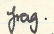
\includegraphics[width=.08\textwidth]{../images/frag.png}};
    \node (m3image) [imageframe , right of=fragimage, xshift=.7cm] {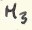
\includegraphics[width=.08\textwidth]{../images/m3.png}};
    \node (azurelabel) [textcontainer, below of=imagelabel, yshift=.5cm] {OCR output};
    \node (frag) [textcontainer, right of=azurelabel, xshift=1cm] {frag.};
    \node (m3) [textcontainer, right of=frag, xshift=.7cm] {H3};
    \node (toothornot) [nnmodel, below of=frag, xshift=1.2cm, yshift=.5cm] {tooth or other?};
    \node (uplow) [nnmodel, below of=toothornot] {upper or lower?};
    \node (mpic) [nnmodel, below of=uplow] {M, P, I or C?};
    \node (mindex) [nnmodel, below of=mpic, xshift=-1.8cm] {1, 2 or 3?};
    \node (pindex) [nnmodel, below of=mpic, xshift=1.8cm] {1, 2, 3 or 4?};
    \node (end) [textcontainer, below of=mpic, yshift=-1.5cm] {frag. m3};

    \draw [arrow, draw=Blue] (frag) -- (toothornot);
    \draw [arrow] (m3) -- (toothornot);
    \draw [arrow] (toothornot) -- node[anchor=east] {tooth} (uplow);
    \draw [arrow] (uplow) -- node[anchor=east] {lower} (mpic);
    \draw [arrow] (mpic) --  node[anchor=east, yshift=0.2cm] {m} (mindex);
    \draw [nonactivearrow] (mpic) -- (pindex);
    \draw [arrow] (mindex) -- node[anchor=east, yshift=-0.2cm] {m3} (end);
    \draw [nonactivearrow] (pindex) -- (end);
    \draw [nonactivearrow] (mindex) -- (end);
    \draw[thick, draw=Blue] (toothornot) -- node[anchor=south] {other} (-1.7,-2) -- (-1.7,-8);
    \draw[->, thick, draw=Blue] (-1.7,-8) -- (2.7,-8);
    \draw[thick, draw=Maroon!30] (mpic) -- (8.5,-5) -- (8.5,-8);
    \draw[->, thick, draw=Maroon!30] (8.5,-8) -- (4.7,-8);
\end{tikzpicture}
    \caption{Flowchart of the proposed tooth recognition pipeline}
    \label{fig:pipeline}
\end{figure}

For all words, bounding boxes and reading results detected by Azure Vision on the element column, the word is first classified to tooth marking or other word.
To constrain the input data to the downstream model, this is completed 
with a regular expression checking whether the reading result of the word consists of a letter and number, or only the 
letter C. Once more robust classifiers are built, this part can be replaced with another deciding 
heuristic, allowing a more variety in tooth notation images to be cleaned. The regular expression 
only recognizes a small fraction due to frequent errors in bounding box detection.

The images of the words recognized as tooth markings are given to a binary image classifier deciding whether the tooth 
is upper or lower jaw and then to a model recognizing if the tooth type is molar, premolar or incisor: as 
canines lack the number and are recognized as teeth only when the Azure Vision result is a letter C, there is 
no need to re-classify the tooth marking as a canine. It should be noted that as soon as the regular expression
heuristic is replaced with anything more complex, the fourth class has most likely to be added to the tooth type classifier.
Once type is decided, the tooth marking image is given to the appropriate index number model. Finally, 
the three pieces of information obtained, jaw, type and number, are combined as the digital tooth marking 
notation. As the final step, all words in the element column are concatenated, and all found teeth are 
collected as a tuple to the tooth records column.

To minimize required manual verification, additional confidence information is added 
to each tooth marking. As each classifier produces the probability of the image containing the 
chosen class as a side result, this probability can be saved as a confidence score. The confidence is taken 
per element description phrase (such as 'much of R. mandible ($\text{P}_4$ - $\text{M}_3$)') by taking the minimum over all 
model confidence scores obtained during inference for the tooth records. For example, if in the 
example description every other decision would be of 100\% confidence but the second tooth being a molar 
would only have 70\% confidence, the confidence of the entire row would be 70\%. This conservative approach is 
due to the costliness of errors: one needs to be absolutely certain before data can be left without manual 
verification.

Next, details related to building the classifiers presented in this section are specified.

\subsection{Building the models}
\label{sect:building-models}

% so now we know we need these models: restate models. now we choose what to try when building them
% list subsubsections, these are the aspects

For the dental marking recognition pipeline, four classifiers are needed: upper or lower jaw, 
tooth type, and two downstream index number classifiers. The experimental 
section considers design decisions for setting up experiments to build these models with maximal accuracy:
 data preprocessing and augmentation along with base model,
transfer learning method and hyperparameter selection. After a presentation of  how the training dataset was created, these aspects are considered.

\subsubsection{Creating the training dataset}

% how i got the data
% Data was extracted from scans by getting bounding boxes from Azure Vision API,
% finding the correct column (nature of specimen or element), and cropping the image 
% according to bounding boxes.
% multiple catalogues used to create training set to get versatile notation
The dataset with a total of 1\,105 images was extracted from the fossil 
catalogues using the first two steps on the pipeline in Figure~\ref{fig:pipeline}:
for each word under the element describing header, the Azure Vision output was classified 
to tooth or other with the regular expression, and 
images with tooth notation were cropped out from the catalogue. Along with the image, the 
Azure Vision \cite{azurevision} reading result was saved. To have as versatile notation as possible, images were 
extracted from several catalogues.

% dataset creation and data balancing
% train and val from same catalogues, test set from new one to hopefully introduce concept drift
%     train on train, model select on val, report accuracy on test set -> true not best but more so worse case generalization accuracy, get that high u real good
% give sample counts after balancing
After extraction, data balancing and splitting to training, testing and validation sets 
was completed.
% with the splitting ratiosTODO give ratios here. TODO give reason for ratio: granularity of validation/test error 
%(how much val/test error decreases if one classification mistake is made)
Because incisors and canines were much more rare 
than molars and premolars in the catalogues, some of the former were manually cropped out 
of catalogues to achieve more variety. After this, sample count differences 
 between the most frequent class and others was computed, and augmented 
images were saved for other classes to make sample counts per class equal. The augmentation 
was implemented using a random rotation of -5 to 5 degrees and a random crop with scale 0.9 to 1.0.
Train, validation and test split was selected by creating a validation dataset of roughly 200 samples to
 not change test error by more than 0.5\% with one sample classification
change. For the test set, 100 samples were kept. This resulted in 
train set sizes, including the images generated to balance classes, of 905 samples for upper or lower, 
2\,071 for M, P or I, 1\,521 for index one to three, and 2\,026 for index number one to four.

% labeling:
% mpi, index number: assume that azure reading is correct where reading is a valid tooth notation
% if incorrect, leave out label and handlabel (dont throw out since these are the hard cases and are valuable!)
% up low: hand label with binary label 0 for low 1 for up, -1 for undecipherable
%     why an undecipherable class:
%     - undecipherable upper/lower: the correct answer is not any of the two, so false or correct classification is equally bad, so accuracy does not fully reflect if the model works perfectly or not.
%     - forcing model to think something a human cannot classify should contain some traits where it could figure which one it is is false and will confuse the model -> worse results
For data labeling, outputs from Azure Vision were heavily utilized. For 
tooth types and index numbers, if the reading result was a valid class, it was assumed to 
be correct and used as a label, saving a significant amount of labeling effort. As the 
images were saved in class-specific directories according to the PyTorch ImageFolder interface,
the correctness of labels could easily be verified by visual inspection. Upper and lower jaw labeling 
was completed manually with a ternary label, zero noting lower, one upper, and -1 an undecipherable jaw.
The undecipherable class was included as there were images where the jaw could not be decided by a human annotator, 
and therefore the correct answer for such an instance would be 'unknown'. Forcing these to be either upper or lower jaw 
would distort the classification task: perfect accuracy would be an undesirable result as the model should 
make mistakes with the undecipherable samples, and the undecipherables would confuse the model as it is required to find signals on why 
the notation is either jaw when none are to be found. Therefore, images with undecipherable jaw side were not given 
to the classifier.

As the work was completed under a non-disclosure agreement, the training datasets were not 
published. As the problem ended up being an interesting task from the perspective of optical character recognition, 
bringing even parts of the catalogue scans available for researchers and machine learning hobbyists is encouraged as it could prove
 valuable both for improving digitized data quality and advancing character recognition techniques.
 
A small sample of the training dataset of premolars is presented in Figure~\ref{image:samples}.

\begin{figure}[h]
    \centering
    \includegraphics*[scale=.5]{../images/trainingsamples.png}
    \caption{Samples from the training dataset for tooth type classification of premolar markings.}
    \label{image:samples}
\end{figure}

\subsubsection{Data preprocessing}
 
% 1 paragraph: denoising and grayscaling
Preprocessing of training, validation and test images was completed by grayscaling, denoising and resizing.
As color channels in images have no meaning for the text on the image, grayscaling was implemented by
 stacking three identical grayscale images
to match the three-channel input size required by the base models.
Denoising was implemented due to
small paper texture shadow and eraser smudge noise with the most basic routine, a Gaussian filter.
The kernel size 3 was chosen by experimentation and visual inspection. Finally, the images were resized to 
ImageNet image size of 224x224 pixels using bilinear interpolation.
No further preprocessing was implemented to keep the images alike the source domain, ImageNet images with real-world noise.
 A catalogue sample before and after preprocessing can 
be found in Figure~\ref{image:noise}.

\begin{figure}[h]
    \centering
    \resizebox{\linewidth}{!}{%
        \begin{minipage}[b]{0.45\linewidth}
            \centering
            \includegraphics*[scale=0.67]{../images/noise.png}
        \end{minipage}
        \hspace{0.5cm}
        \begin{minipage}[b]{0.45\linewidth}
            \centering
            \includegraphics*[scale=0.67]{../images/denoised.png}
        \end{minipage}
    }
    \caption{A catalogue sample with paper texture shadow and eraser smudge noise before and after grayscaling and denoising.}
    \label{image:noise}
\end{figure}

% 3. tested but not implemented things
% segmenting out the letter: does not make sense since the premise of deep learning is 
% to to feature extraction better than a human would do. to segment out the letter you would 
% need to know which area is the letter and to know that you need to know what letter there 
% is which is the problem in the first place, so unsolvable egg hen problem. show some example from preprocessing notebook

% no binarizing: some letters are super weak text so theyd get lost and some background clutter might be dark.
% popular was wan thresholding but im not confident in this case where intensities change so much you could 
% do any deterministic binarization
More heavy preprocessing steps of binarization and extracting only the letter or number from the image were 
attempted but not implemented.
Binarizing the images was considered as evidence was found for that to increase result accuracy~\cite{9thuonPalm},
but was not implemented since the noise, in many cases
 parts of neighboring characters due to bounding box errors, are occasionally of darker 
color than the correct text, making thresholding difficult. Additionally,
 initial experiments with a MNIST base model suggested the resulting
accuracies were decreasing when using binary input images. However, binarization scheme was not designed carefully 
and the experimentation was not exhaustive.
Another aspect considered after binarizing was to try to segment out the letter for the tooth type recognizer 
and the number to the index number recognizer, but it was found that there was so much variability 
among the images that implementing a deterministic algorithm was hard. 
As the premise of deep learning is that such challenging feature extraction becomes unnecessary as the neural 
network is better at extracting relevant information than a human designing preprocessing routines~\cite{princebook}, these 
heavier preprocessing operations were not used.

\subsubsection{Data augmentation}
\label{sect:aug}

% paragraph 1: augmentation routines were chosen to mimic what could happen really
% how i will augment: those that might happen in scanning process
% intensity value change (idk scanner illuminates differently)
% change background and letter contrast (some paper is lighter than other)
% random cropping (to mimic bounding box detection errors, dont translate bc that creates the white background that never occur in test data)
% minor rotation (up to 5 degrees, scanner does not turn that much and handwriting is generally pretty straight)
% horizontal and vertical shear to mimic different handwriting styles
Data augmentation operations were chosen according to variation that can 
occur among scans of documents with handwriting.
Due to paper and pen color differences, functions on pixel intensity
values were applied to adjust brightness and contrast by using the 
TorchVision ColorJitter transformation with brightness factor range from 
0.95 to 1.05 and contrast factor range from 0.8 to 1.2. To mimic bounding box detection errors, 
a random crop was implemented using RandomResizedCrop with 
scale from 0.9 to 1.0 to not crop out significant parts of the character but 
still introduce cropping variation. Rotation from -5 to 5 degrees 
was implemented as some tables were sligtly tilted in the scan images. 
Lastly, handwriting variation was mimiced with horizontal and vertical 
shear by setting shear ranges for both horizontal and vertical directions from 1 
to 10 pixels with the RandomAffine operation. The background was filled in 
with white after rotation when necessary to match the other background as closely as possible.
 A batch of training images after augmentation
is presented in Figure~\ref{image:augmented}.

\begin{figure}[h]
    \centering
    \includegraphics*[scale=.2]{../images/augmented.png}
    \caption{Samples of the training dataset after data augmentation.}
    \label{image:augmented}
\end{figure}

\subsubsection{Base model selection}

% 1. paragraph: verification of hypothesis that imagenet indeed was the best
% According to~\cite{emnistclassifiersurvey}, this model was the best:~\cite{jamilemnist}, was chosen as the base model.
% they trained on emnist-balanced, so no difference between upper -and lower case letters. not a problem for us since 
% in the handwritten catalogues, upper or lowercase was not used to distinguish upper and lower jaw

% mnist and real world fundamental difference: mnist is perfect world, real images vary much more~\cite{alexnet}
% therefore: not e(mnist) as source problem, but imagenet classification.

To select appropriate base models, one first needs to select the source task and domain. Since most reviewed work uses image classification as the source task, this is assumed to work best.
Another potential source task would have been the identity mapping task given to the autoencoder,
but it was not implemented due to lesser popularity and the small size of the dental marking image dataset.
As the source domain, there are two datasets used in previous work: the classification of digits in the MNIST dataset, 
and the ILSVRC classification challenge with the ImageNet dataset. The popular 
assumption that ImageNet is a better source domain was verified with a short experiment by training a MNIST classifier~\cite{jamilemnist}
to classify tooth types with best accuracy of 89\%, that was clearly outperformed by the ImageNet-based classifiers. This verifies the commonly assumed hypothesis that real-world images of any objects is a more 
similar domain than the MNIST dataset of handwritten digits, which is known to contain ideal-case images with little noise.

% 2 paragraph: selection of base models based on previous work
% Chosen public dataset was EMNIST~\cite{emnist} because it is the closest to my problem: a large dataset of labeled letters and numbers.
The ImageNet classifier base models used in this the experiments are selected 
according to results from related work, reviewed in Section~\ref{sect:same_solution}.
The models were chosen by checking which base models 
occurred multiple times when listing the top three models in terms of accuracy. 
Analyzing Table~\ref{tab:model-info}, EfficientNet models \cite{efficientnetv2} consistently outperform 
other architectures, most often with the V2S variant, closely followed by the 16-layer variant of the VGG architecture~\cite{vgg},
DenseNet121 \cite{densenet}, and ResNet101 \cite{resnet}.
Therefore, these four architectures were chosen as base models.
Additionally, the Vision Transformer \cite{vit} and AlexNet \cite{alexnet} were included, the former to test 
transformer architectures on the fossil domain and latter
as proof-of-concept experiments suggested high accuracy scores.
The shortcoming in this base model selection is that as previous work did not give much
 reasoning for their base model selection, it is possible that some high-performing architectures were not included 
because  they were not chosen to be experimented with. As one has to limit the 
search space of architectures in some way, previous success was kept as the main deciding heuristic 
even when acknowledging these limitations.

% return to tables 3,4 which base models seemed to work in literature
% those variants that occur many times in top3
% efficientnet
% vgg16
% densenet121
% resnet101
% obvious flaw: no whys in prev work why they chose what they chose but 
% one cannot test everything so we choose these.

\subsubsection{Transfer method selection}

% why i only always keep unfrozen layers after frozen layers
% some papers did some first layer unfreezing, or middle layer unfreezing ie something else 
% but not freezing last layers. dismiss that because 
% they did not state why they did that. from the learn higher and higher level features point of view 
% having an not frozen layer and then after that a frozen one does not make any sense; the later 
% layer is based on the previous. so never in experiments have a frozen layer below a layer that is frozen

% why i start from more frozen to less frozen
% more frozen is less training effort, more generalizable (less is fit to specific data set)
% this is overall better so therefore first this
% if the search space of parameters is too small (model converges to low accuracy), freeze one layer by one 
% until overfits: training error is much larger than test error. sign: we trained too many parameters / for too long

% small dataset -> train less layers to not overfit to the target dataset
For transfer method selection, the reviewed work in Table~\ref{tab:model-info} has a variety of approaches, 
the only common trend being that freezing less seems to be beneficial. 
However, how much to freeze is very dependent on transfer distance and target data size;
freezing more should work in cases very similar as the features should be more useful 
and in cases of small target data, where overfitting is avoided.
For these reasons it is argued that transfer method selection should be
based on experimentation rather than previous results.

For the choice of which layers to freeze, layers will be only frozen so that a frozen layer never 
occurs after a trainable layer. This is because of the assumption that high-level layers 
encode generic and lower layers more specific features, and the generic features are assumed to be most transferable among tasks.
 Additionally, as specific features build on the generic ones, freezing layers 
below ones modified is assumed to confuse the model. Thus, all experiments consist of some layers 
at the start of the network being frozen and others at the end being open for updates.
The number of trained layers is used to specify the transfer method 
for each experiment, and these are always the last layers of the network.

As another experimentation principle, the trials will start out from settings where more layers are frozen, proceeding to
cases where more parameters can be updated. This is because more freezing saves 
computational effort, and is less likely to overfit to the training set as there is a lesser degree of freedom 
available for updating parameters. Therefore, it is sensible to look for the model that re-uses as 
much parameters as possible but still has enough flexibility to find a good optimum for the target problem:
this is assumed to result in the best generalization capability.

\subsubsection{Hyperparameter selection}

% fix hyperparameters: do not experiment with too much at a time.
% Take hyperparameters that were most common among reviewed re.
As for hyperparameters, values are selected according to well-performing 
options in reviewed literature to scope down the experimentation search space.
Hyperparameter tuning was not implemented to keep experimentation 
between approaches fair; if the optimization is better for some case than other, one can no 
longer deduce whether the difference in result accuracy was due to hyperparameter or base model and 
transfer approach optimality. Therefore, hyperparameters are fixed between experiments to common values 
used previously in similar tasks. The selected hyperparameters, most chosen mostly by popularity 
with the only exceptions of reducing number of epochs as experiments converged early
and adding learning rate scheduling to aid optimization,
are summarized in Table~\ref{table:hyperparameters}.

\begin{table}[h!]
    \centering
    \caption{Hyperparameters used in the experiments.}
    \begin{tabular}{ll}
    \hline
    \textbf{Hyperparameter} & \textbf{Value} \\ \hline
    Batch size & 64 \\ 
    Number of epochs & 20 \\
    Optimizer & Stochastic Gradient Descent with Momentum \\
    Momentum & 0.9 \\
    Learning rate & 0.001 \\
    Learning rate scheduler & Step (multiply by gamma=0.1 every 7 epochs)\\
    Loss function & Categorical cross-entropy \\ \hline
    \end{tabular}
    \label{table:hyperparameters}
\end{table}

% the hyperparameters

% image normalization mean and std (for numerical stability of training (doublecheck this is the reason!))
% batch size 
% num epochs 
% optimizer 
% learning rate 
% learning rate scheduling
% loss function
% many runs and final accuracy averaging; how many runs

% For each: list what papers used generally, pick a nice average value
% then i tested with the best model these to check sensitivity to hyperparameter choice, so 
% robustness of optimization. esp change the random seed to see results dont depend on that
%     but so the hyperparam sensitivity thing:
%         if the experiment results hold across a population -> which method works best should work best in all 
%             hyperparametrizations and not only in this one. vary hyperparameters and check if comparison 
%                 (which was better than which) still holds
%         differences in accuracy are due to the hyperparameters being more optimal in some cases than some 
%             you can never really eliminate this 
%             one should further verify how robust the experiments are to hyperparameter changes
%             I can test around a little bit to check that my some better than some holds at least in most cases

% % summary of chapter
% this chapter gave an overview of how the experiments were set up and why they were set up in this way.
% a sentence from all: sequence not done bc its complex. multiclass not done bc it is worse according to~\cite{tibetan_ocr}.
% training setting: preprocessing by denoising only because nn premise is that the net is better at feature extraction than human.
% augmentation: intensity change background contrast change random crop letter blur minor rotation because these can happen in catalogue scans
% base models are: efficientnet vgg16 densenet121 resnet101 because they were popular and or won comparing benchmarks in previous work
% freezing first more then less bc if more works its better, find sweet spot of most freezing that is still accurate.
In this chapter, the experimental setup along with reasoning for design decisions were given.
In the problem formulation, classifying words with a chain of univariate classifiers was opted for to 
maximize the accuracy by simplifying the problem as far as possible.
Preprocessing was kept minimal with denoising and grayscaling, 
and augmentation was set up to variations that might occur in the scanning process. Base models were mostly
chosen according to previous success, resulting in selecting the EfficientNetV2S, VGG16, DenseNet121, ResNet101, ViT and AlexNet architectures.
Transfer methods are compared by experimentation: the model with most layers frozen while still being able to find a good optimum 
for the target task is searched for. In the next chapter, 
results from these experiments are presented and evaluated.

\section{Results and discussion}

% introduction to chapter
% present the results from experiments
% % start of section: reiterate what was experimented with
% guidepost to discussion
% first evaluation of result, its strengths and shortcomings
% then discussion on if comparing architectures makes sense in a small data case
% last discussion on what this might tell about transfer learning theory. why it works
This chapter presents the results of the experiments. The comparative experiments were completed using the 
upper and lower jaw classification problem, since initial experiments suggested it to be the most challenging 
classification task. The experimentation was limited to testing out different base models, AlexNet, EfficientNet, 
DenseNet, Vision Transformer and Resnet, and freezing setups: training 1, 5, 10 or all layers.
The results of these experiments highlighted three major results. First, the best architectures were AlexNet and the Vision 
Transformer with best validation accuracies of 92,21 and 91,56, respectively, while EfficientNet performed poorly. Second, tests on changes in results 
when adjusting hyperparameters suggested that comparisons of model architectures should be taken with caution since one can never know 
if the differences in end accuracy were due to differences in model architecture or in how good the found optimum was 
for the network parameters. Lastly, as the strongest result it is found that freezing less 
always increases resulting accuracy, and it is discussed whether this suggests that it is better to interpret transfer learning as extended 
training rather than a re-use of feature extraction. These aspects are discussed in more detail in this chapter. After this, future work 
suggestions are presented, informed by the outcomes of this study.

% GENERALIZATION CAPABILITY / QUALITY OF MY RESULTS
% quickly refer the table
% 	vit: 2nd, so don't forget about transformers, but don't forget about cnn's either. both seem to work almost equally well.
% train test dirrecence max 8.59 but most in 0-3\% range. so: very similar train test accs, so: generalizes well
% initial hypo of freeze more to overfit less does not seem to hold: no larger train val acc differences with less freezing
The experiment outcomes are collected to Table~\ref{table:results}, and 
the most important findings are the following. Using AlexNet as the base model results in the highest 
validation accuracy with the Vision Transformer as a close second. Having the transformer 
architecture not as the best but still a competitive result verifies the result 
from another study that stated CNNs to outperform transformers, but suggests 
that transformer architectures are worth testing for in building various OCR
solutions. Another interesting point is that EfficientNet results were the worst of all, 
which strongly contradicts results of many reviewed works in Section~\ref{sect:same_solution},
suggesting that a model found to be better in one study can inform little on its performance on another target task.
The generalization capability of all models seems to be good, as seen in Figure~\ref{image:diff_hist}:
the difference between training and validation accuracies is in the majority of 
experiments below 4 \%. As there is little correlation between the magnitude of this difference, 
a metric for degree of overfitting, and layers trained, the initial hypothesis on freezing more to prevent overfitting
seemed to not hold.

\begin{table}[ht]
    \centering
        \begin{tabular}{|c|c|c|c|}
            \hline
            \textbf{Training Accuracy (\%)} & \textbf{Validation Accuracy (\%)} & \textbf{Layers Trained} & \textbf{Base Model} \\ \hline
            92.71 & $\mathbf{92.21}$ & all  & AlexNet~\cite{alexnet}       \\\hline
            90.83 & 88.96 & 10   & AlexNet~\cite{alexnet}      \\\hline
            84.30 & 80.52 & 5    & AlexNet~\cite{alexnet}      \\\hline
            64.09 & 61.69 & 1    & AlexNet~\cite{alexnet}      \\\hline
            95.25 & $\mathbf{91.56}$ & all  & ViT ~\cite{vit}         \\\hline
            68.84 & 66.88 & 10   & ViT ~\cite{vit}         \\\hline
            68.73 & 64.94 & 5    & ViT ~\cite{vit}         \\\hline
            50.06 & 42.86 & 1    & ViT ~\cite{vit}         \\\hline
            90.72 & $\mathbf{87.01}$ & all  & VGG16    ~\cite{vgg}    \\\hline
            84.31 & 80.52 & 10   & VGG16  ~\cite{vgg}      \\\hline
            72.27 & 67.53 & 5    & VGG16  ~\cite{vgg}      \\\hline
            43.65 & 35.06 & 1    & VGG16  ~\cite{vgg}      \\\hline
            88.73 & 81.17 & all  & DenseNet121~\cite{densenet}  \\\hline
            66.08 & 65.58 & 10   & DenseNet121~\cite{densenet}  \\\hline
            65.75 & 65.58 & 5    & DenseNet121~\cite{densenet}  \\\hline
            55.80 & 62.34 & 1    & DenseNet121~\cite{densenet}  \\\hline
            64.75 & 65.58 & all  & ResNet101 ~\cite{resnet}   \\ \hline
            64.75 & 65.58 & 10   & ResNet101  ~\cite{resnet}  \\\hline
            64.75 & 65.58 & 5    & ResNet101 ~\cite{resnet}   \\\hline
            60.77 & 63.64 & 1    & ResNet101 ~\cite{resnet}   \\\hline
            64.53 & 64.29 & all  & EfficientNetV2S ~\cite{efficientnetv2} \\\hline
            64.09 & 64.29 & 10   & EfficientNetV2S~\cite{efficientnetv2}  \\\hline
            64.09 & 64.29 & 5    & EfficientNetV2S~\cite{efficientnetv2}  \\\hline
            54.59 & 54.55 & 1    & EfficientNetV2S~\cite{efficientnetv2} \\\hline
        \end{tabular}
    \caption{Training and Validation Accuracy for Different Base Models and Layer Freezing setups for Upper / Lower jaw classification}
    \label{table:results}
\end{table}

\begin{figure}[h]
    \centering
    \includegraphics*[scale=0.7]{../images/train_val_error_difference_histogram.png}
    \caption{Histogram of percentage-point differences in training and validation accuracies within each experiment}
    \label{image:diff_hist}
\end{figure}

% RANDOM SEED / HYPERPARAMETER SENSITIVITY: ON THE FLIMSEYNESS OF MODEL ARCHITECTURE COMPARISONS
% sensitivity to hyperparams/random seed? tested by setting seed from 15 to 2 8 (random choice) and re running for alexnet.
% 	there is room for hyperparameter optimization
% 	it was still the case that more freezing worse result
% 	random seed essentially determines how the data points are divided into batches. batch division that happens to be better for optimization can lead to a better optimum and a better model. emphasis: model comparison is hard, margin of error is up to 10\% where you should not be too sure the better model is actually better
% 	so, if one does model comparisons then it is important that the hyperparameter search is actually exhaustive, you actually try every single seed so each model has the best seed used. practical thing is, you can never really do that. therefore model comparisons should be done with caution.
% 	this also means that doing proper experimentation is quite expensive computationally, luckily small data transfer learning is not that cpu intensive.
% theres no metric for quality of optimum found.
% to actually compare architectures you'd nee
% many h param setups, compare each and check if one is best in eeevery case
% but: cpu intense.
% we see here efficientnet was very unsuitable -> architecture comparison paper contribution is not necessarily that relevant bc the information is not generalizable
% 	best model in one is not the best in other is at least proven for sure.
% random seed: shows that initial examples are very important in finding a good optimum!

To estimate how much the results depended on the optimum found in training and how much on the architecture, 
the best architecture AlexNet was retrained with one hyperparameter changed, and the resulting 
change in accuracy suggests that comparing architectures when target data is small is highly inaccurate. 
A change in the random seed from 15 to 2, both randomly chosen, was done to check how much the result changes 
when the only thing changed is the order of training samples in batches. This changes which initial examples are shown to the model,
changing the initial steps of the learning trajectory, which is important in neural network training~\cite{transferlearning_survey}.
 As seen in Table~\ref{table:random_seed_sensitivity}, the largest difference occurred with one layer 
trained, and the second seed had the validation accuracy increased by 9,09 percentage points. This shows that initial examples 
are important and can initialize much better or worse learning trajectories. Then, hyperparameter change 
by changing batch size from 64 to 32, also a random choice, was tested with the AlexNet architecture, and the results 
changed by 6,49\%, as seen in Table~\ref{table:hyperparameter_sensitivity}. Notably, the best accuracy was outperformed by as much as 4,54 percentage points 
in this setting, more than halving the count of errors. These large variances serve as a good example on the caveats of comparing 
base models in a small target data transfer setting: since there is no objective metric for the quality of optimization, there 
is practically no way of knowing what the true reason for accuracy differences between experiments is. In this case, the 
margin of error can be approximated at 10\%, that is, only when validation accuracies differ by more than that one can be 
somewhat confident that the better result actually has a superior architecture. Taking this into account, AlexNet, ViT and VGG16 
can all be considered best-performing architectures in this study. Having access to more validation data or more computational 
resources to repeat the experiments with different hyperparameter settings would be required to draw more fine-grained conclusions on the 
superiority of an architecture over another.

\begin{table}[ht]
    \centering
        \begin{tabular}{|c|c|c|c|}
            \hline
            \textbf{Accuracy, first seed (\%)} & \textbf{Accuracy, second seed (\%)} & \textbf{Difference (\%)} & \textbf{Layers Trained} \\ \hline
            88.31 & 92.21 & 3.9  & all \\\hline
            85.71 & 88.96 & 3.25 & 10  \\\hline
            75.32 & 80.52 & 5.2  & 5   \\\hline
            52.60 & 61.69 & 9.09 & 1   \\\hline
        \end{tabular}
    \caption{Random seed sensitivity: validation accuracies with two different seed values}
    \label{table:random_seed_sensitivity}
\end{table}

\begin{table}[ht]
    \centering
        \begin{tabular}{|c|c|c|c|}
            \hline
            \textbf{Accuracy, batch size 64 (\%)} & \textbf{Accuracy, batch size 32 (\%)} & \textbf{Difference} (\%) & \textbf{Layers Trained} \\ \hline
            92.21 & 96.75 & 4.54 & all \\\hline
            88.96 & 93.51 & 4.55 & 10  \\\hline
            80.52 & 87.01 & 6.49 & 5   \\\hline
            61.69 & 61.69 & 0 & 1   \\\hline
        \end{tabular}
    \caption{Hyperparameter sensitivity: validation accuracies with batch sizes 64 and 32}
    \label{table:hyperparameter_sensitivity}
\end{table}

% IS TRANSFER LEARNING JUST MORE TRAINING?
%no freezing was best. observations.
% no freezing was best (see the plots, this held in every single experiment so very strong result)
% result aligns with other ocr studies.
% resnet and efficientnet: maybe all information on the training dataset was able to be encoded to the first five layers and therefore more unfreezing did not provide more value
% train the last layer (inspo from~\cite{4zhaoTibetan}, hypothesis of reusing feature extractor as is seems false, training the whole network works better.
The clearest result from the experiments is that freezing never improved the resulting accuracy. This result was 
also the only larger consensus among studies reviewed in Section~\ref{sect:same_solution}.
As is highlighted in the plot of layers trained against resulting accuracy in Figure~\ref{image:accuracy_vs_freezing},
there were no exceptions to this relationship. Accuracy of DenseNet and ResNet plateauing can be seen as 
the model having enough freedom to encode all information present in the training data and therefore adding 
more trainable parameters did not increase accuracy. To interpret the correlation, the hypothesis that using a feature 
extractor as is, inspired by the Tibetan glyph classification solution~\cite{4zhaoTibetan}, did not result in the 
best model in the fossil domain; additional feature tuning was needed.

\begin{figure}[h]
    \centering
    \includegraphics*[scale=0.8]{../images/accuracy_against_freezing.png}
    \caption{Line plots of accuracy scores with different freezing setups reveal the positive correlation of accuracy and count of layers trained}
    \label{image:accuracy_vs_freezing}
\end{figure}

% mnist or imagenet as a base model
% initial phase experiments: mnist transfer to mpi since it was thought to be a similar problem. 
% mnist had worse result 89\% with quick testing, above-90 never achieved w. mnist
% imagenet is more similar than mnist: real world image classification is much more complex than digit classification~\cite{alexnet}
% mnist shortcoming: benchmark images are ideal cases with eg perfectly even background. 
% also~\cite{8goelGujarati2023} had the same result (that imagenet is better than mnist even though mnist data looks more like character images)
To analyze transfer distances, less rigorous experiments were implemented on a MNIST base model~\cite{jamilemnist}.
This was implemented to check the hypothesis that transfer distance from MNIST to fossil data is larger than that where 
the base task is ImageNet: even though the former contains characters, the ideal-case benchmark images are more dissimilar 
as they contain no clutter or noise very present in real-world images~\cite{alexnet}. This was found to be true; 
initial experimentation, although not as rigorous as the ImageNet-based experiments, never achieved above-90\% accuracies.
This result was shared by the handwritten Gujarati detection study~\cite{8goelGujarati2023}, where ImageNet as base task 
outperformed MNIST in all layer freezing scenarios. 

%"we need to go further"
% two ways to study: learn principles (encode priors to models/ constrain the problem), show examples of special cases
% transfer learning is good because part of the special case example "studying" was done for you. ofc u need to study something relevant so there transfer distance comes in so you reuse training, not features
% no freezing: more trainable parameters so you can just train more?
% base tasks: imagenet is much larger so more training was done? and therefore imagenet's better?
% --> we need to go further (analogue to the meme)
% --> pick your model, and throw data and compute at the problem as much as you can.
To draw an analogue from neural networks to learning in general, the central lesson learned in these experiments 
is that there is no trickery to learning. To learn something, there are two avenues: one is to learn principles, which in 
neural networks happens by encoding prior information in architectures or constraining the problem space. After that, the only 
option is to repeatably expose the learner to examples. The feature-recycling premise of transfer learning seems to be that 
by reusing features, some of this example study could be circumvented. The fact that freezing always deteriorated performance
raises the hypothesis that this could be untrue, that the real value of transfer learning is that a part of the learning from 
examples is re-used from another training run, allowing for training longer and therefore seeing more examples. Transfer distance 
fits in this with the intuition that all examples seen to learn a trend need to be relevant to the problem. 
Taking the idea that transfer utility is only about 
seeing more examples further, one can even hypothesize whether the superiority of ImageNet over other base tasks, like MNIST, is 
due to the transfer distance being shorter or if the reason is the sheer size of the dataset. Summarizing all this, the lesson learned
can be boiled down to one phrase, inspired by the GoogLeNet inspiring meme presented in 
Figure~\ref{image:meme}, one can simply say "we need to go further"; the way forward is simply exposing the model to more examples, 
and re-using the previously learned as much as possible.

% back to the higher level task of constructing the pipeline: test 
% errors and outcomes of the system
% test errors and certainty scores.
% x why test set
% i don't list validation accuracy as one should not to describe generalization,
% because val accuracy was used to do model selection -> there is data leakage in the validation accuracy
% x what is certainty score.
% a metric for what proportion of samples the model was more than human level ie 99,7 percent certain 
% - c's are a struggle. on the other hand this suggests that the sub/superscript is learned very well, only one such sample
% comparison to generalist
% x judging on how many things i corrected when labeling, this is far better than the generalist.
% x random seed disclaimer: still many percentage points fluctuation
% varied random seed mpi, lowest was bit below 90 so seed variance even here, acc was always 100
% x task comparison follows how hard it felt to label.
% ndex was hardest becuase often esp lower part of number gets cut out -> 2 and 3 distinguising is hard
% - class imbalance thing
% class imbalance was severe in some cases so the less common classes had to be augmented 
% a lot, so could overfit to the small amount of samples, also causes that test err is not necessarily that representative.
Returning to the higher level task, all models presented in Section \ref{sect:pipeline} were constructed, evaluated and used 
in building the inference pipeline. For evaluation, test error was measured on a new set not used in previous experiments 
to prevent data leakage; data used to inform the model building process should never be used to report final accuracies \cite{engbook}.
A certainty score was constructed to measure what fraction of images was classified with above-human accuracy of 99,7\% to measure 
how much manual verifying labor can be saved with the system. The evaluation metrics are presented in Table \ref{tab:task_accuracy_certainty}.
The results align with intuition from the labeling process; labeling images 
where Azure AI Vision \cite{azurevision} had made a mistake felt easiest 
with the letter and hardest for the number, largely due to bounding box errors 
cutting of parts of the digit, often the bottom. Also judging on the labeling experimence,
the results with custom-made models outperforms the generalist, although no 
correctness metrics were counted for the Azure readings. 
As for limitations for these results, results need to 
be taken with caution as varying the random seed caused fluctuations of 
up to 10\% also in evaluation. The test accuracies can also be unaccurate because 
of severe class imbalance especially for the index numbers, where the digit 1 was so few
in number that it is possible that the model has overfit to these examples.
Finally, as seen in Figure \ref{image:misclassifications_uplow_in_test},
the upper and lower jaw classifier struggled to classify canines correctly;
only seven instances like these were present in the test set, five of 
which were misclassified. On the other hand, this also means that other upper 
and lower jaw classifications were learned well. This is suggested by 
the pipeline outcomes: all images tested, albeit a small sample, were 
assigned a correct dental marking. In the aggregated confidence score, 
high individual subtask confidences were undermined by some lower confidences, 
causing most of final confidence scores to be below human-level accuracy, leading 
to possibly only a small amount of saved manual verifying efforts. 
A snapshot of dental markings constructed can be seen in Figure \ref{image:inference}.


\begin{table}[h!]
\centering
\begin{tabular}{|l|c|c|}
\hline
\textbf{Task}       & \textbf{Accuracy (\%)} & \textbf{Certainty (\%)} \\ \hline
MPI                 & 100.00                 & 94.50                   \\ \hline
Upper/Lower         & 92.31                  & 71.79                   \\ \hline
123                 & 88.00                  & 58.00                    \\ \hline
1234                & 91.39                  & 62.92                   \\ \hline
\end{tabular}
\caption{Task Accuracy and Certainty Levels}
\label{tab:task_accuracy_certainty}
\end{table}

\begin{figure}[h]
    \centering
    \includegraphics*[scale=0.8]{../images/misclassified_uplow.png}
    \caption{Samples from the test set falsely classified by the best classifier. The letter C with a line on top or bottom is detected poorly; seven of these were present in the test set.}
    \label{image:misclassifications_uplow_in_test}
\end{figure}

\begin{figure}[h]
    \centering
    \includegraphics*[scale=0.8]{../images/inference.png}
    \caption{Sample outputs of dental notation and associated confidence values. Only few of the samples exceed human-level classification accuracy of 99,7\%.}
    \label{image:inference}
\end{figure}

\subsection{Future work on digitizing fossil catalogues}

% shortcomings; add to 1st paragraph. + add guiding part on what this sect is about
% - i lose context between words ie. mandible with m1-3 we know is lower. sequence based analysis would help here
% - vocabulary-based analysis, the set of words that can occur in a catalogue vs. all words in a
%   language is a very small subset -> good constraint but i did not find a way to encode it to the model
% - best accuracy came from an experiment to test hyperparam sensitivity with a random hyperparam choice ->
%   hyperparam tuning could result in a better accuracy.
% - task dissimilarity to other ocr: extra info on image with character and number. idk if character classification 
%   was the best technique. this needs adjustment anyway to eg. cope with M1-3 multiclass things. that is new in ocr in general: 
%   marking that is many classes at the same time is like a character that would be a b and c at the same time, sign of maybe wrong formalization

% why word bounding box worked badly and how it could be improved
% how this could be continued
% main problem in working with azure bounding boxes: incorrect identification of word bounding boxes.
% encoding prior knowledge should work better: M1-3 is a word for instance, azure did stuff like m, 1-, 3
While this work managed to accurately clean a part of dental markings present in the catalogues, 
there are several potential directions to significantly improve the digitization of such catalogues in general, the main direction 
being improving the quality of word-location defining bounding boxes. The main problem in the bounding boxes provided 
by Azure Vision~\cite{azurevision} was that the dental marking words were often cut across many words or were present 
as a part of a longer word. This is likely due to the space width varying greatly between different pieces of 
handwriting, and sub or superscripts being unfamiliar to the model. To improve the correctness of handwriting segmentation to words, developing a fine-tuned word detector 
could improve the result: a specialist model encoded with knowledge on what kinds of words are more likely to be 
present in the data would likely be much better at finding correct bounding boxes. An example of 
such case is seen in Figure~\ref{image:hardsentence}: a segmenter with the knowledge of tooth marking notation could 
easily see that the $\text{dm}_{3-4}$ section is one word, which is difficult to a generalist model 
due to the spacing between characters.

\begin{figure}[h]
    \centering
    \includegraphics*[scale=0.8]{../images/hardwordsegmentation.png}
    \caption{Example of a sentence hard to segment to words without context knowledge}
    \label{image:hardsentence}
\end{figure}

% point of this paragraph: object detection is a harder task and has gotten attention from cv research in recent years.
% on hardness. from computer vision lecture 11~\cite{ruotsalainen2024}
% object bounding box detection requires higher resolution images and ground truth labels -> labeling effort is 
% big, compute needed. one idea is to take premade bounding boxes by generalist ocr word detectors and for example
% infer they are correct by matching with a vocabulary of known correct words to exist in fossil catalogues.
% pointers to research work on computer vision object detection
% on recent work. several new advances seem without testing promising, but unfortunately their main problem is differnet from ours so not directly applicable
%I quickly tested a state of the art object detection model the yolo10, variant of popular object detector yolo\cite{redmonYouOnlyLook2016}
%  untuned, on huggingface api, the yolo10~\cite{OmouredYOLOv10DocumentLayoutAnalysisHugging2023}. The performance 
% was poor, see fig, probably since object detection usually does 3d object detection in a 3d scene, so one should either 
% fine tune or find a ocr bounding box detector. then there is open-vocabulary object detector which you can tell what objects 
% are present~\cite{YOLOWorldRealTimeOpenVocabulary}. we could just say there are teeth and words. 
% then also a very recent publication on detecting text on images~\cite{longHierarchicalTextSpotter2024}.
% benefit of these is that they are fine-tunable which the commercial azure api is not. 
% then also detectron~\cite{Detectron} from meta for object detection
% one could also run more sophisticated 
% tooth or not classification on azure output, which could work very well but relying on a paid service is not ideal 
% for open access solutions.
The problem of finding objects in images is much harder than image classification and has attracted attention 
from the computer vision research community very recently. 
Main reasons for the difficulty are the labour required to obtain ground truth bounding boxes and 
the fact that object detection requires better image resolution to work well, therefore requiring more computational resources~\cite{ruotsalainen2024}.
One way to circumvent manual annotation for fossil catalogues could be to automatically detect correct bounding boxes 
from commercial OCR engine output files for instance by regular expression matching the word readings with a vocabulary of words likely to be 
present in fossil catalogues, much like the approach implemented in this work.
For the detection model, several recent advances seem promising, but might not be directly applicable without fine-tuning 
due to the fact that the standard problem of object detection is to detect three-dimensional objects in 3D scenes, which is 
quite different from word detection on a flat, scanned document. This is likely the reason why an initial experiment 
ran on the Hugging Face API version~\cite{OmouredYOLOv10DocumentLayoutAnalysisHugging2023} of YOLO-10~\cite{wang2024yolov10}, a variant of the highly influential object detector YOLO~\cite{redmonYouOnlyLook2016},
resulted in a very poor segmentation found in Figure~\ref{image:yolo}: the entire image was segmented as one object.
Some possibly more applicable models, however not as easily testable due to lesser popularity, 
are the open-vocabulary version of YOLO~\cite{YOLOWorldRealTimeOpenVocabulary},
 the hierachical text spotter~\cite{longHierarchicalTextSpotter2024}, and the Detectron by Meta~\cite{Detectron}.
 However, due to the catalogue-specific problem illustrated in Figure~\ref{image:hardsentence}, it is likely that these 
 models would require well-optimized fine-tuning to work well. It is also possible that from 3D to scan image transfer distance is 
 too large and OCR-specific object detectors need to be found. Experimenting with such implementations is a 
 substantial effort and was omitted from this work to keep the scope reasonable.

% % improving MPI/upperlower classification (not as hard so not as relevant perhaps)
% ways to improve the result of image classification obtained here 
% test svm after feature extraction instead of the dense layers + softmax. My most recent model was from (insert year),
% since then imagenet classification has advanced, so try using a newer base model. these can be harder to obtain 
% since they are not as established, I could just fetch models from torchvision.models, newer ones are not present there.
% with a good object detector probably we can get to more variaty of tooth marking images (maybe a fig of examples?)
% so the classification task would become more complicated. Still, the downstream tooth marking image to tooth task 
% is a relatively easy classification problem comparing to eg imagenet, so the main challenge is definitely finding words and
% classifying them to tooth or not.
Another possible line of extending the work would be improving the accuracy of the image classification to tooth type. 
Some ideas include to extend the model with capabilities of detecting markings with multiple teeth, although
a rather unusual case of multi-class character classification, and to experiment with more recent ImageNet classifiers with better top-5 and top-1 error rates.
However, using the newer models would require more effort since good pretrained weights are 
more difficult to find for the less established models, and there is less evidence of their applicability to downstream tasks.
Improving the model would still be highly useful, since a more sophisticated word object recognizer would result in a more 
variable set of tooth marking images to be given to the tooth type classifier, making its classifying problem much more difficult. 
Still, the object detection problem should be given more attention since even the 
potential harder variants the dental marking classification task are relatively simple image classification problems when comparing 
them to challenges such as basic ImageNet classification.

\begin{figure}[h]
    \centering
    \includegraphics*[scale=0.3]{../images/yoloresult.png}
    \caption{Preliminary object detection test with the YOLO-10 object detector using the Hugging Face inference API~\cite{OmouredYOLOv10DocumentLayoutAnalysisHugging2023}.}
    \label{image:yolo}
\end{figure}

\section{Conclusions}

Returning from the problem of digitizing handwritten fossil specimens to the larger picture, several thoughts arose on the potential of centralized, structured databases for paleontological research from several short conversations with practicioners.
These ideas can be seen as a reiteration on what was attempted in this thesis, or toward which goal a tiny step was made. For any large endeavor one needs a 'north star', a guiding goal, to inform the direction of developing the methods. Looking from the perspective of a data scientist, it seems that the north star for paleontological databases is very much obtainable and holds a large potential for saving lots of routine work for much more meaningful activities. To conclude this work, these ideas are explored; what could be possible, what the utility of such a tool would be, and what it would take to develop one.

To see what could be, a good analogue to start from is that of scientific journals. If those were what fossil data largely is like today, journals would be scattered around the world, some saved digitally, some in paper form. Should someone want to study a subject, the work would start from finding where interesting material could reside, traveling to the location and saving photocopies of physical and copies of digital work. The very possible future scenario for fossil data would be like Google Scholar is for research: one search box, where a researcher wishing to analyze a subject could write, for instance, 'all lower third molars globally, with all loph counts, dated and with location', and a dataset could be created in seconds. The English-accepting search box is more of a fancy feature, an ordinary SQL database with querying access globally would do much of the same job; requiring users just to learn a few basic SQL commands. With a bit less simple database, a multimodal database could store 3D images of the physical samples along with each data entry. Setting specific features aside, the main point is that a dramatically more convenient data storage is not utopian; the techological tools exists and are routinely used in other domains.

The NOW database~\cite{Žliobaitė2023} is perhaps the closest example of a structured fossil database, but upon a quick look still has lots of improvements to be made. The most obvious is to collect more specimens there, and expanding from mammals to all other forms of life as well. From a governance perspective, a truly all-encompassing database should be even more global in the administrating team, and the copies of the database could well be stored in multiple locations globally. The data scheme, without seeing the backend, seems to be built with a species as the main data unit. A more suitable one could be logging each specimen find as one data point, as these represent the smallest 'atom' of data in this context. These could then be linked to a species. The user interface of the NOW database is quite clear, but in this use case a text interface would be much more suitable than a graphical one: a database has so many commands that constructing a form and buttons for each leads to a cluttered and inevitably limited-capability interface. A textual interface with a single command prompt, accepting a database language such as SQL or even natural language should one build an english-to-sql tool for this case, would simplify the interface to what google.com looks like, while providing every imaginable database function. Of course, the user interface or data scheme design of a paleontological database service could be the topic of another thesis, and cannot be covered in depth here.

The Google Scholar analogue likely highlighted already what the utility of a global, all-encompassing paleontological database could be, but several more benefits should be covered. To state the obvious, huge amounts of tedious and boring data acquisition and uniformizing effort could be saved, and this saved time could then be spent conducting more research, thinking deeply about the analytical problems, or simply not working at all. Another type of work that could be saved significantly is that of data creation: if every measurement and taxon identification, after completed, could be saved indefinitely and for everyone to access, no measuring would be done twice. Additionally, when saving new measurements, the result tractability could be improved with metadata: the person completing the measurement, date, and any thoughts regarding the measurement could be saved. Should any doubts of the correctness of a measure or taxon identification arise, this data or the person could be consulted, and the data corrected if necessary. Versioning schemes could be designed to save a history of these corrections. Should one want to see the physical samples, the database still had an utility of serving as a search engine for finding where relevant specimens reside. Lastly, this much more standardized approach to fossil data would allow much better reproducibility: the database query to get the dataset used in each study could be published, and the data could be obtained by anyone evaluating the study to re-run or further experiment with the analysis conducted. With these changes in habits of data management, the actual thing that matters, the quality of knowledge on the distant past, could be dramatically improved.

What it would take to get to this state of data quality would mostly be just to work; much of the technological tools already exist. For digitizing, as completed in this thesis, well-established practices go a long way. Fossil data has its specialities as an optical character recognition problem, but is mostly a rather conventional problem.
What would be required from paleontologists is a standard of measurement: what should be measured, and in which units, which should then be used in every study working with the common traits. For the database creation, as already brushed on, software design, data versioning and management aspects need to be considered. Still, a large hurdle is the amount of work and collaboration required for storing all data globally in one database. There needs to be an incentive for someone, who already conducted the analysis, to undergo the additional effort of sending out the measurements collected for the study for further use, as this effort does not directly benefit the sender in any way. An expectation for everyone to do this could suffice. As is known by all natural scientists, species that collaborate flourish, and it is in the interest of everyone to do what one can to advance the field in general.

\printbibliography
\end{document}